\documentclass[12pt]{report}
\usepackage[a4paper, width=150mm,top=25mm,bottom=25mm]{geometry}
\usepackage[utf8]{inputenc}
\usepackage{blindtext}
\usepackage{graphicx}
\usepackage{lipsum}
\usepackage{times}
\usepackage{titlesec}
\usepackage{tocloft}
\usepackage{pdfpages}
\usepackage{amsmath}
\usepackage{listings}
\usepackage{xcolor}
\usepackage{tikz}
\usepackage{pgf-umlcd}
\usepackage{caption}
\usepackage{subcaption}
\usepackage[colorlinks=true,linkcolor=black,urlcolor=black,citecolor=black]{hyperref}
\usetikzlibrary{positioning, shapes.geometric, arrows,calc,arrows.meta}
\graphicspath{{images/}}

% Define block styles
\tikzstyle{block} = [rectangle, draw, fill=blue!20, 
    text width=5em, text centered, rounded corners, minimum height=4em]
\tikzstyle{sum} = [draw, fill=blue!20, circle, minimum size=1cm, node distance=1.5cm]
\tikzstyle{input} = [coordinate]
\tikzstyle{output} = [coordinate]
\tikzstyle{pidblock} = [draw, dashed, inner sep=0.5cm, rounded corners]

% Define custom colors
\definecolor{mygreen}{rgb}{0,0.6,0}
\definecolor{mygray}{rgb}{0.5,0.5,0.5}
\definecolor{mymauve}{rgb}{0.58,0,0.82}
\definecolor{backcolour}{rgb}{0.95,0.95,0.92}

% Set up listings for MATLAB, Python, and C
\lstset{ 
    backgroundcolor=\color{backcolour},   % choose the background color
    basicstyle=\ttfamily\footnotesize,  % the size of the fonts that are used for the code
    breakatwhitespace=false,         % sets if automatic breaks should only happen at whitespace
    breaklines=true,                 % sets automatic line breaking
    captionpos=b,                    % sets the caption-position to bottom
    frame=single,                    % adds a frame around the code
    keepspaces=true,                 % keeps spaces in text, useful for keeping indentation
    numbers=left,                    % where to put the line-numbers
    numbersep=5pt,                   % how far the line-numbers are from the code
    numberstyle=\tiny\color{mygray}, % the style that is used for the line-numbers
    rulecolor=\color{black},         % if not set, the frame-color may be changed on line-breaks within not-black text (e.g. comments (green here))
    showspaces=false,                % show spaces adding particular underscores
    showstringspaces=false,          % underline spaces within strings
    showtabs=false,                  % show tabs within strings adding particular underscores
    tabsize=2,                       % sets default tabsize to 2 spaces
    title=\lstname                   % show the filename of files included with \lstinputlisting; also try caption instead of title
}

% MATLAB settings
\lstdefinestyle{MATLAB}{
    language=Matlab,
    keywordstyle=\color{blue},
    commentstyle=\color{mygreen},
    stringstyle=\color{mymauve}
}

% Python settings
\lstdefinestyle{Python}{
    language=Python,
    keywordstyle=\color{blue},
    commentstyle=\color{mygreen},
    stringstyle=\color{mymauve}
}

% C settings
\lstdefinestyle{C}{
    language=C,
    keywordstyle=\color{blue},
    commentstyle=\color{mygreen},
    stringstyle=\color{mymauve}
}

\renewcommand{\cftchapleader}{\cftdotfill{\cftdotsep}} 
\renewcommand{\cftchapfont}{\normalfont\bfseries}

\newcommand{\name}{Shashank Agarwal}
\newcommand{\faculty}{Dr.Loveleen Kaur Taneja}
\newcommand{\industry}{Mr.Sarv Parteek Singh}
\newcommand{\director}{Mr.M.S. Saini}

\begin{document}
\begin{titlepage}
    \begin{center}
        
\includegraphics{university.png}\\
        {\textbf{Project Report}}\\
        \vspace*{0.2cm}
        (Internship Semester January--June)

        \vspace*{3cm}
        {\Large\textbf {Design of Front end converter using SVPWM technique}}

        \vfill
        Submitted by

        \vfill
        \textbf{
        \name \\
        21104027
        }

        \vfill
        Under the Guidance of
    \end{center}
    \vfill

    \noindent
    
    \begin{minipage}[t]{0.5\textwidth}
        \raggedright
        \industry \\
        Technical Advisor\\
        Statcon Electronics India Ltd,\\
        Noida
    \end{minipage}
    \hfill
    \begin{minipage}[t]{0.5\textwidth}
        \raggedleft
        \faculty \\
        Faculty Coordinator\\
        Department of Electical Engineering\\
        Punjab Engineering College (Deemed to be University),\\
        Chandigarh
    \end{minipage}
\end{titlepage}

\includepdf[pages={1}]{Intern Certificate.pdf}
\setlength{\parindent}{0pt}
\pagenumbering{roman}

\titleformat{\chapter}[display]
{\normalfont\huge\bfseries\centering}{\thechapter.}{20pt}{\Large}

\chapter*{Declaration}
I hereby declare that the project work entitled "Design of Active Front End" is
an authentic record of my own work carried out at Statcon Electronics India Ltd
as requirements of six months project semester for the award of degree of
B.E./B.Tech. Electrical Engineering, Punjab Engineering College (Deemed to be
University), Chandigarh, under the guidance of \industry\ and \faculty, during
January to June, 2024.

\vspace*{2.5cm}
\noindent
\begin{minipage}[t]{0.5\textwidth}
    \raggedright
    {Date: {\today}}
\end{minipage}
\hfill
\begin{minipage}[t]{0.5\textwidth}
    \raggedleft{
        \name \\
        21104027
    }

\end{minipage}
\vfill

\noindent
Certified that the above statement made by the student is correct to the best of our knowledge and belief.

\vspace*{2cm}

\noindent
\begin{minipage}[t]{0.5\textwidth}
    \raggedright
    \faculty \\
    Faculty Coordinator\\
    Department of Electical Engineering\\
    Punjab Engineering College (Deemed to be University),\\
    Chandigarh
\end{minipage}
\hfill
\begin{minipage}[t]{0.5\textwidth}
    \raggedleft
    \industry \\
    Technical Advisor\\
    Statcon Electronics India Ltd,\\
    Noida

\end{minipage}

\chapter*{Acknowledgement}
\input{chapters/acknowledgement}

\titleformat{\chapter}[hang]
{\normalfont\LARGE\bfseries}{\thechapter.}{20pt}{\LARGE}

\tableofcontents
\listoffigures

\clearpage
\pagenumbering{arabic}

\chapter{Summary}
I got the opportunity to do my internship at Statcon Electronics India Ltd.
Statcon Electronics established in 1986 is one of India's largest ISO
9001-20151 certified manufacturer of Static energy Conversion system. During my
internship at Satcon Electronics India Ltd, Noida, I was first assigned to
explore Space Vector Modulation technique and then make a simulation for a
front end converter using Space Vector Modulation. I was part of the Embedded
Software team and my task was to develop a control algorithm for the front end
converter.\\

The aim of the project to design a Active Front End converter for a Hybrid
inverter,aiming to enhance its efficiency and performance while reducing
harmonic distortions and improving the power factor.

\section{Timeline}
My internship at Statcon Electronics India Ltd started on 10th January, 2024.
My mentor gave me the task of exploring Space Vector Modulation and developing
control algorithm for the front end converter. This timeline will briefly
explain the course of my internship from beginning to end.

\subsection{January}
In January, I started learning about Space Vector Pulse Width Modulation
(SVPWM). This involved understanding two important things: the Clarke and Park
transforms. These transforms help to change three-phase voltages into a simpler
two-dimensional form, making it easier to control three-phase systems. The
Clarke transform turns three-phase voltages into two-phase parts, while the
Park transform changes these parts into a fixed frame of reference. I also
learned about space vectors, which show how the three-phase voltages combine.
This knowledge helped me understand SVPWM better. It's a technique that uses
space vectors to control how inverters produce voltage. This exploration gave
me a better grasp of how SVPWM works and its uses in power electronics.

\subsection{Feburary}
During February, I immersed myself in the study of the Clarke and Park
transforms, essential mathematical tools used in analyzing three-phase
electrical systems.The Clarke transform simplifies three-phase voltages into
two-phase components, making it easier to understand and analyze complex
electrical systems. Similarly, the Park transform further refines these
components into a fixed frame of reference, streamlining the analysis and
control of electrical signals. Alongside theoretical exploration, I practically
experimented by developing Python code to implement and test these
transformations. This hands-on approach not only deepened my understanding of
the transforms but also provided valuable insights into their real-world
applications and implementation challenges.

\subsection{March}

During March, I worked on developing and testing a three-phase Phase-Locked
Loop (PLL) algorithm using Python. This algorithm used the Clarke and Park
transforms to precisely estimate the angle of the space vector in the
three-phase system. Following the initial testing phase of the PLL algorithm in
Python, I transitioned to Simulink/MATLAB for further simulation. Within the
Simulink environment, I used MATLAB function blocks to implement the PLL
algorithm. Once this was completed, I proceeded to make a three-phase inverter
in Simulink using IGBT components. Leveraging MATLAB function blocks and the
output of the PLL, I then generated gate timing signals for the Front end of
the inverter, ensuring precise control and synchronization of the electrical
signals.

\subsection{April}

In April, I worked toward fine-tuning the Proportional-Integral (PI) controller
for the Phase-Locked Loop (PLL) using the Ziegler–Nichols method. This involved
adjusting the parameters of the PI controller to optimize the performance of
the PLL algorithm. By employing the Ziegler–Nichols method, I aimed to achieve
stability and responsiveness in tracking and synchronizing the phase of
electrical signals effectively. Additionally, I implemented a control loop in
MATLAB function blocks to measure the current flowing from the front end to the
grid. This control loop allowed for the adjustment of the output voltage to
either draw or supply the desired current, depending on the system
requirements.

\subsection{May}
In May, I completed the simulation and proceeded with the actual implementation
of the front end on hardware. I began by selecting a suitable microcontroller
with DSP capability, opting for the STM32F411 microcontroller. Then, I
initiated the coding process, developing functions for voltage transformations,
PID controller, and Phase Lock Loop (PLL). Additionally, I integrated unit
testing using Unity to test individual functions of the code. Moreover, I
created a native target to provide sample signals to the code, generating
output graphs for viewing. This approach allowed me to test my code without the
need for a microcontroller.

\subsection{June}
In June, I relocated from the Noida office to the Hyderabad office to continue
developing both the code and hardware. While in Hyderabad, I familiarized
myself with the standard coding structure required for our projects and
proceeded with the development process.

I began writing the code for the microcontroller, During this phase, I learned
about Direct Memory Access (DMA) and interrupts, which I used to sample the
input voltage. Using these sampled voltages as reference values, I generated
the Space Vector output in the form of Pulse Width Modulation (PWM) signals
from the microcontroller. This approach ensured precise and efficient control
of the system.
\chapter{Introduction}
An active front-end (AFE) converter, is a grid interface converter that
transfers power between an energy source and the utility grid, and between the
utility grid and a load. It's a controllable rectifier that can exchange power
between AC and DC power in both directions, and can regenerate power to the
mains to reduce power costs.
\section{Problem Statement}
My team at Statcon Electronics India Ltd has been focusing on on enhancing the
efficiency and performance of front-end converters. Presently, most active
front-end converters utilize Silicon Controlled Rectifiers (SCRs) for
rectification, employing a conventional 6-pulse converter configuration. My
task was to explore and design a active front-end using Insulated Gate Bipolar
Transistors (IGBTs) as alternatives to SCRs in the rectification process.\\

The primary objective of this project is to investigate the feasibility and
advantages of using IGBTs instead of SCRs for rectification in active front-end
converters. Specifically, we aim to implement a Space Vector Pulse Width
Modulation (SVPWM) technique to control the IGBTs effectively. This technique
offers precise control over the switching patterns of the IGBTs, allowing for
optimized power conversion and reduced harmonic distortion.\\

Furthermore, the project involves the development of a sophisticated control
algorithm to manage the operation of the IGBTs. This algorithm must facilitate
seamless transition between pulling current from the grid (rectification mode)
and supplying current to the grid (regeneration mode). The control system
should ensure stable and efficient operation under varying load conditions
while maintaining compliance with grid standards and regulations.

\section{Overview}
A three-phase AC to DC converter is essential for many power electronics system
such as Variable frequency drive (VFD), battery charger, uninterruptible power
supplies (UPS).

Traditionally diode rectifiers or thyristor rectifier are used for AC to DC
conversion, both these rectifiers behave as non- linear loads. The currents
drawn by the rectifiers include a fundamental component and harmonic
components. The voltage drop across the line inductance due to the harmonic
currents distorts the mains voltage. Consequently, the other loads connected to
the mains are also fed with a distorted voltage.

\subsection{Traditional Rectifier}
Diode rectifier, depicted in Figure~\ref{fig:diode_rectifier}, produces a
constant DC voltage, which is a function of the system voltage. A thyristor
based rectifier can produce a variable DC voltage. But, both these topology
behave as non-linear loads.

\begin{figure}[h]
    \centering
    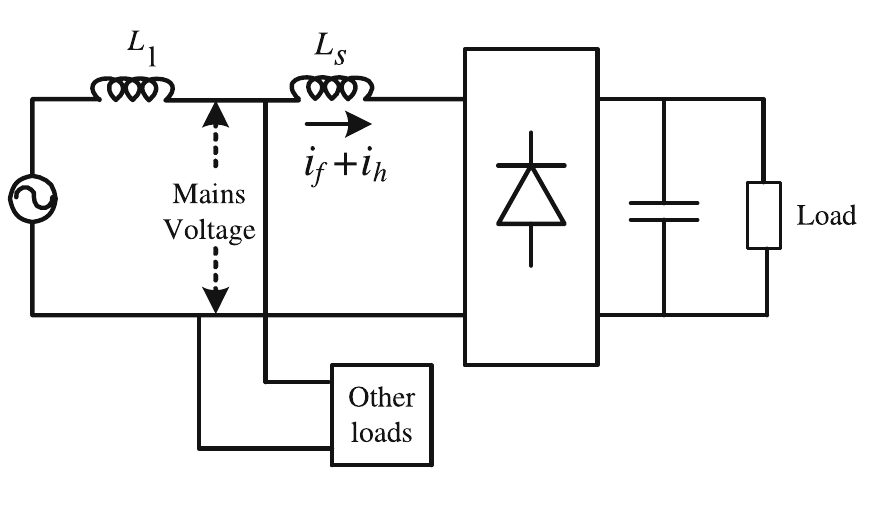
\includegraphics[width=\textwidth]{Diode Rectifier.png}
    \caption{AC to DC Conversion using Diode Rectifier.}
    \label{fig:diode_rectifier}
\end{figure}

\subsection{IGBT Rectifier}
\begin{figure}[h]
    \centering
    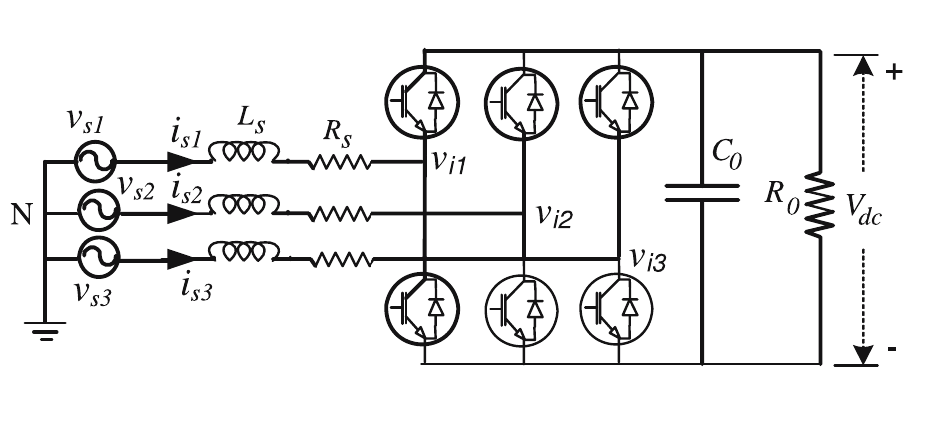
\includegraphics[width=\textwidth]{IGBT Rectifer.png}
    \caption{Schematic diagram of
        a front-end converter (FEC)}
    \label{fig:igbt_rectifier}
\end{figure}
\noindent
IGBT Rectifer, depicted in Figure~\ref{fig:igbt_rectifier}, draws near
sinusoidal current from grid. The power factor as well as DC Voltage can be
adjusted. Since it is connected to line side it is called line side or front
end converter.

The converter consists of a three-phase bridge, a high capacitance on the dc
side and a three-phase inductor in the line-side. The voltage at the mid point,
$V_i$ is pulse width modulated (PWM) in nature. The voltage consists of a
fundamental component (at line frequency) besides harmonic components around
the switching frequency of the converter. Being at high frequencies, these
harmonic components are well filtered by the line inductor. Hence the current
is near sinusoidal. The fundamental component of $V_i$ controls the flow of
real and reactive power.

\subsection{Vector Control}
Vector control is a popular method for control of three-phase induction motors.
The basic idea of this scheme is to control the flux producing and the
torque-producing components of motor current. The outer control loop controls
the speed of the motor, while the inner loop controls the components of current
vector, which correspond to torque and flux. Similar control approach can be
used for FEC also. Here, the three-phase grid voltages and line currents are
converted into an equivalent two-phase system, called stationary reference
frame . These quantities are further transformed into
a reference frame called synchronous reference frame, which revolves at the
grid frequency .

\subsection{Space Vector Modulation}
This technique, also known as Space Vector Pulse Width Modulation (SVPWM), is a
method used to generate the switching signals for the IGBTs in the AFE
converter. It offers precise control over the IGBT switching patterns by
synthesizing the desired output voltage as a combination of multiple voltage
vectors. SVM has eight space vectors, other space vectors are synthesized by
alternating active and zero vectors over a switching period.

\section{Challenges}
I faced many challenges in developing a Active front-end converter. Firstly,
distinguishing between Sinusoidal Pulse Width Modulation (SPWM) and Space
Vector Pulse Width Modulation (SVPWM) posed confusion due to their perceived
similarity in operational principles. Secondly, reconciling the non-zero
resultant vector in SVPWM with the traditional understanding of three-phase
systems, where the vector sum equals zero, required conceptual clarification to
ensure accurate system design and analysis. Another challenge was comprehending
how rectification and regeneration can occur through the same IGBT bridge, as
it involved bidirectional power flow management. Additionally, not knowing how
to write code in MATLAB was another challenge, but learning it opened up new
possibilities for simulating and analyzing our AFE converter designs.
\chapter{Work}
\section{Simulation}
\begin{figure}[h]
    \centering
    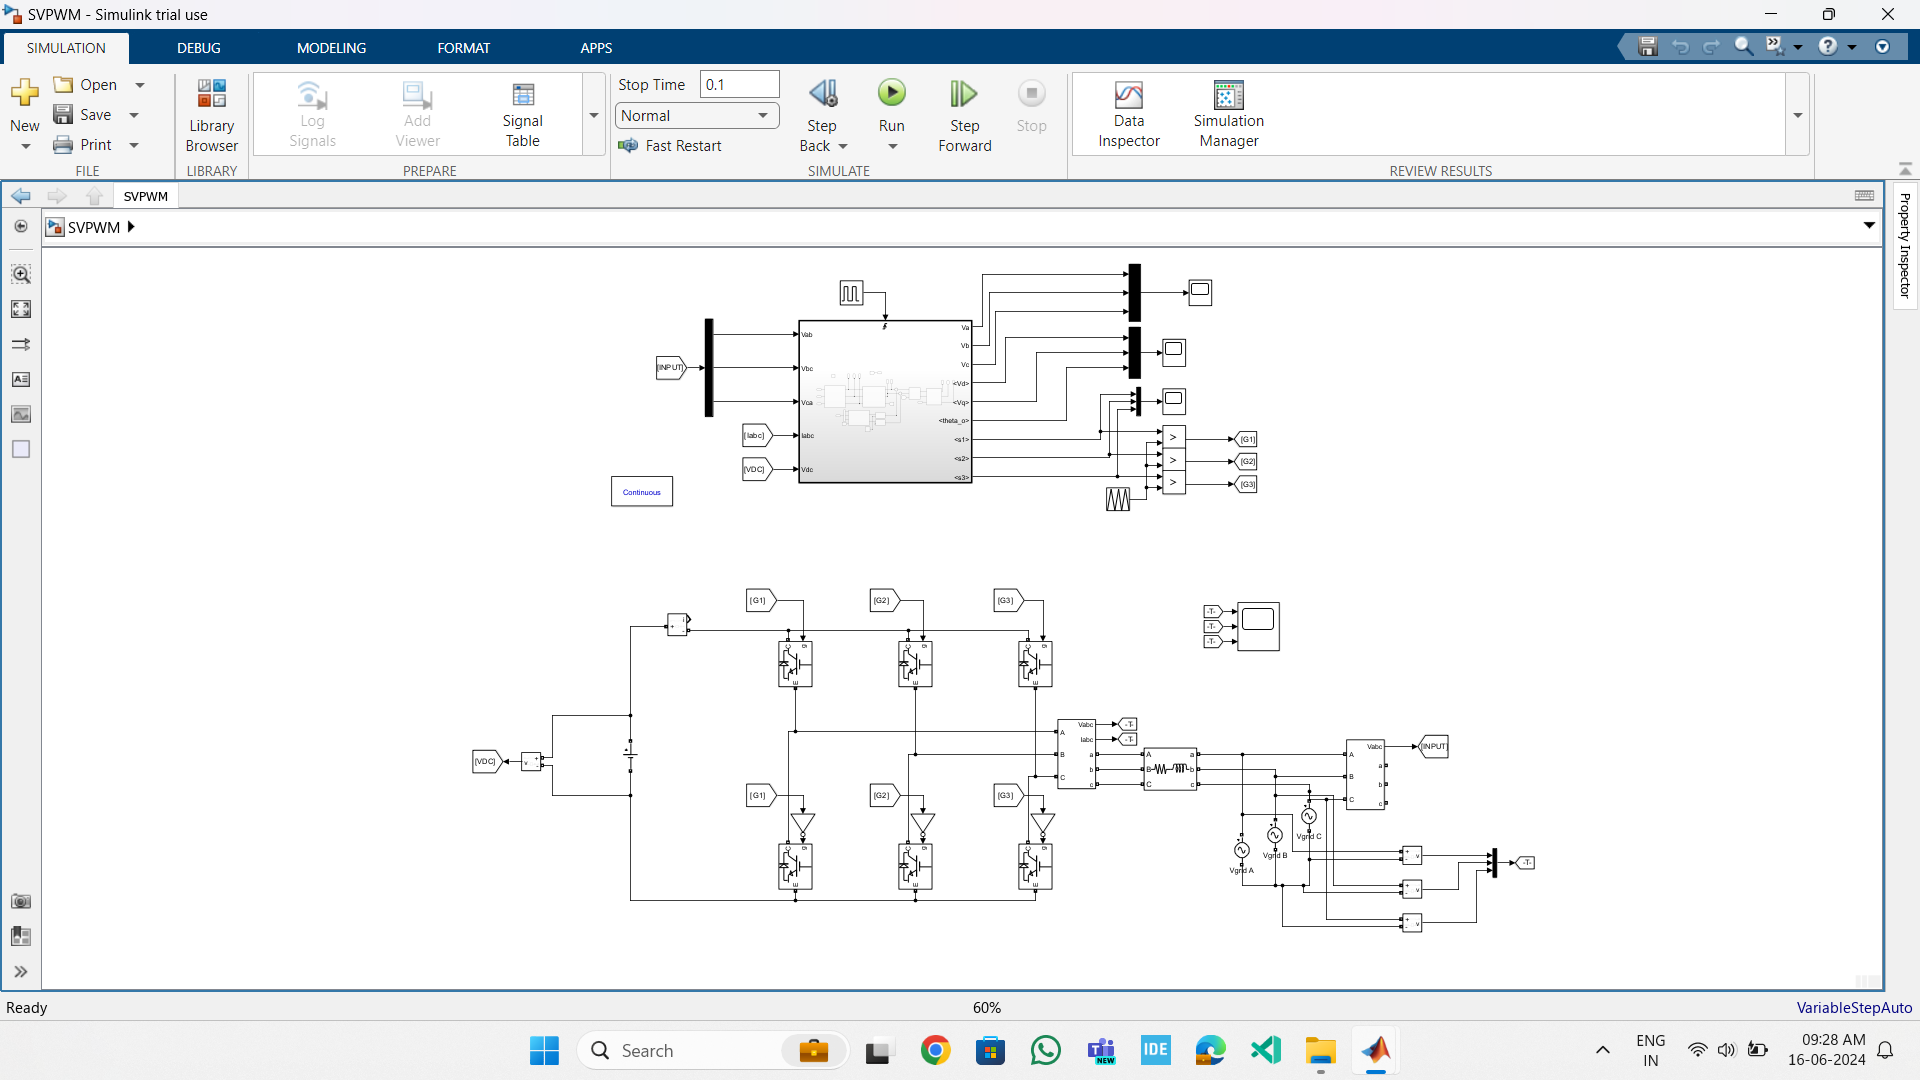
\includegraphics[width=\textwidth]{Whole Simulation.png}
    \caption{Simulation}
    \label{fig:Simulation}
\end{figure}
Before initiating the implementation phase, it was imperative to conduct a
comprehensive simulation of the front end using Simulink/MATLAB. The simulation
setup involved importing a three-phase source from MATLAB and configuring the
necessary parameters for voltage and current measurements.

\subsection{MATLAB Function Blocks in Simulation}
To emulate the behavior of a microcontroller in the simulation environment,
MATLAB function blocks were extensively utilized. These function blocks
provided a familiar coding environment, resembling the programming paradigms
employed in microcontroller firmware development. By encapsulating custom
algorithms and control logic within MATLAB function blocks, it was possible to
simulate complex control strategies and signal processing techniques with ease.
This approach not only facilitated rapid prototyping and testing but also
provided invaluable insights into the real-time behavior of the system. The use
of MATLAB function blocks bridged the gap between simulation and
implementation, enabling seamless transition from design validation to hardware
deployment.
\subsection{Control System}
\begin{figure}[h]
    \centering
    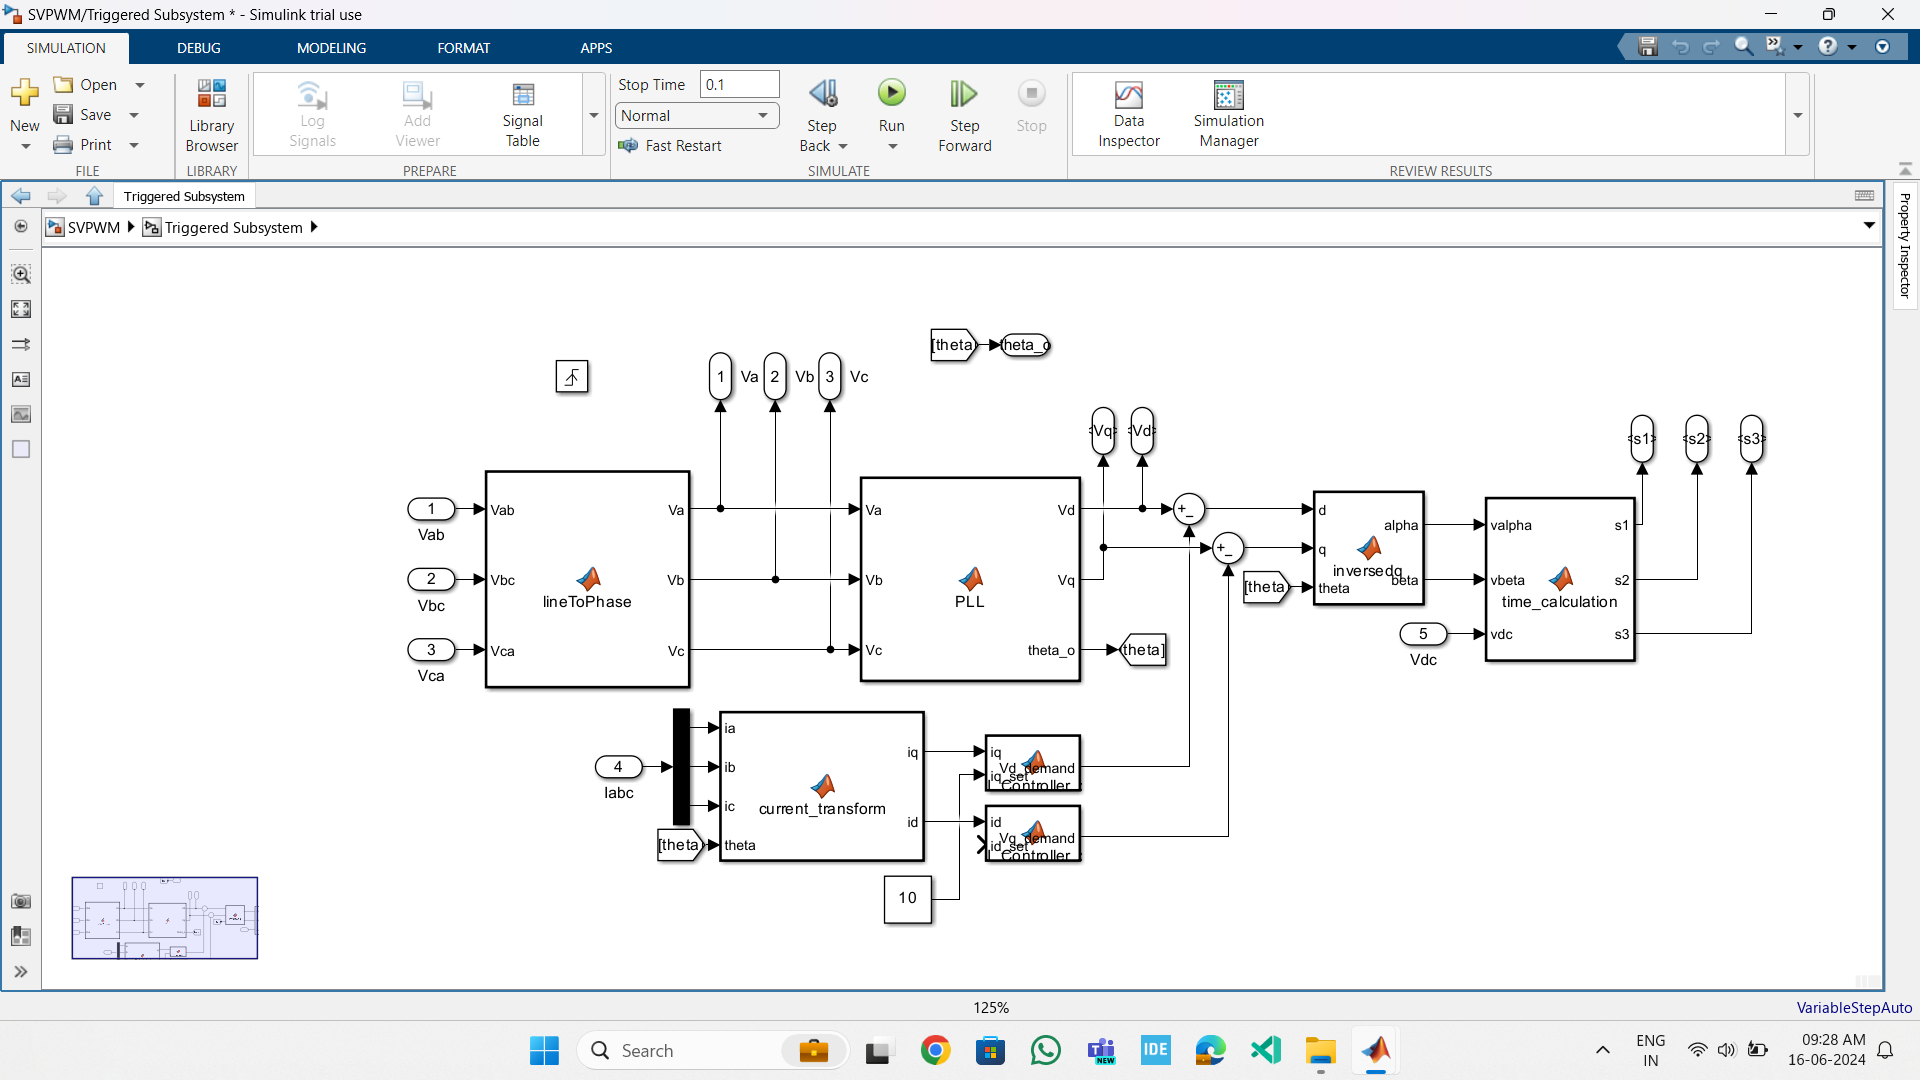
\includegraphics[width=\textwidth]{Control flow.png}
    \caption{Control System}
    \label{fig:Control System}
\end{figure}
\subsubsection{Voltage Transformation}
Transform the measured line voltages from the three-phase source into the
alpha-beta frame using the Clarke transform. This transformation facilitates
easier analysis and control of the three-phase system. The Clarke transform
converts three-phase voltages into two orthogonal components (alpha and beta),
simplifying the analysis of the system's dynamics and making it easier to
implement control strategies.

\subsubsection{Phase-Locked Loop (PLL)}
Incorporate a Phase-Locked Loop (PLL) block to convert the voltages from the
alpha-beta frame to the dq rotating reference frame. Additionally, the PLL
provides the angle theta of the voltage vector, crucial for subsequent control
strategies. The PLL ensures synchronization with the grid by maintaining a
constant phase relationship, which is vital for accurate control and stability
of the system.

\subsubsection{Current Measurement and Transformation}
Measure the line current flowing into the front end, and using Clarke and Park
transform blocks, convert it to the dq reference frame. Utilize the angle theta
obtained from the PLL for this transformation. The dq reference frame allows
for decoupled control of the direct and quadrature components of the current,
enabling more precise control of the active and reactive power.

\subsubsection{Current Regulation}
Regulate the current flowing into the front end to ensure stable operation and
adherence to system constraints. Employ two Proportional-Integral (PI)
controllers to compare the measured current to a predetermined set current
value and generate control signals for current regulation. The PI controllers
adjust the control signals to minimize the error between the measured and
desired current values, ensuring the system operates within the desired
parameters.

\subsubsection{Voltage Calculation and Transformation}
Add the control signals (delta Vq and delta Vd) obtained from the PI
controllers to the Vq and Vd components obtained from the PLL. Convert these
voltages back to the Clarke frame using the inverse Park transform. This step
integrates the control efforts with the system's voltages, transforming the
controlled voltages back into the stationary reference frame for further
processing and application.

\subsubsection{Gate Timing Calculation}
Utilize the voltages calculated in the previous step (V alpha* and V beta*) to
determine gate timings for the three-phase active front end. These gate timings
dictate the switching patterns of the Insulated Gate Bipolar Transistors
(IGBTs), essential for controlling the flow of current through the front end.
The precise timing of the IGBT switching is crucial for maintaining the desired
current and voltage waveforms, ensuring efficient and stable operation of the
power conversion system.

\subsection{Power System}
\begin{figure}[h]
    \centering
    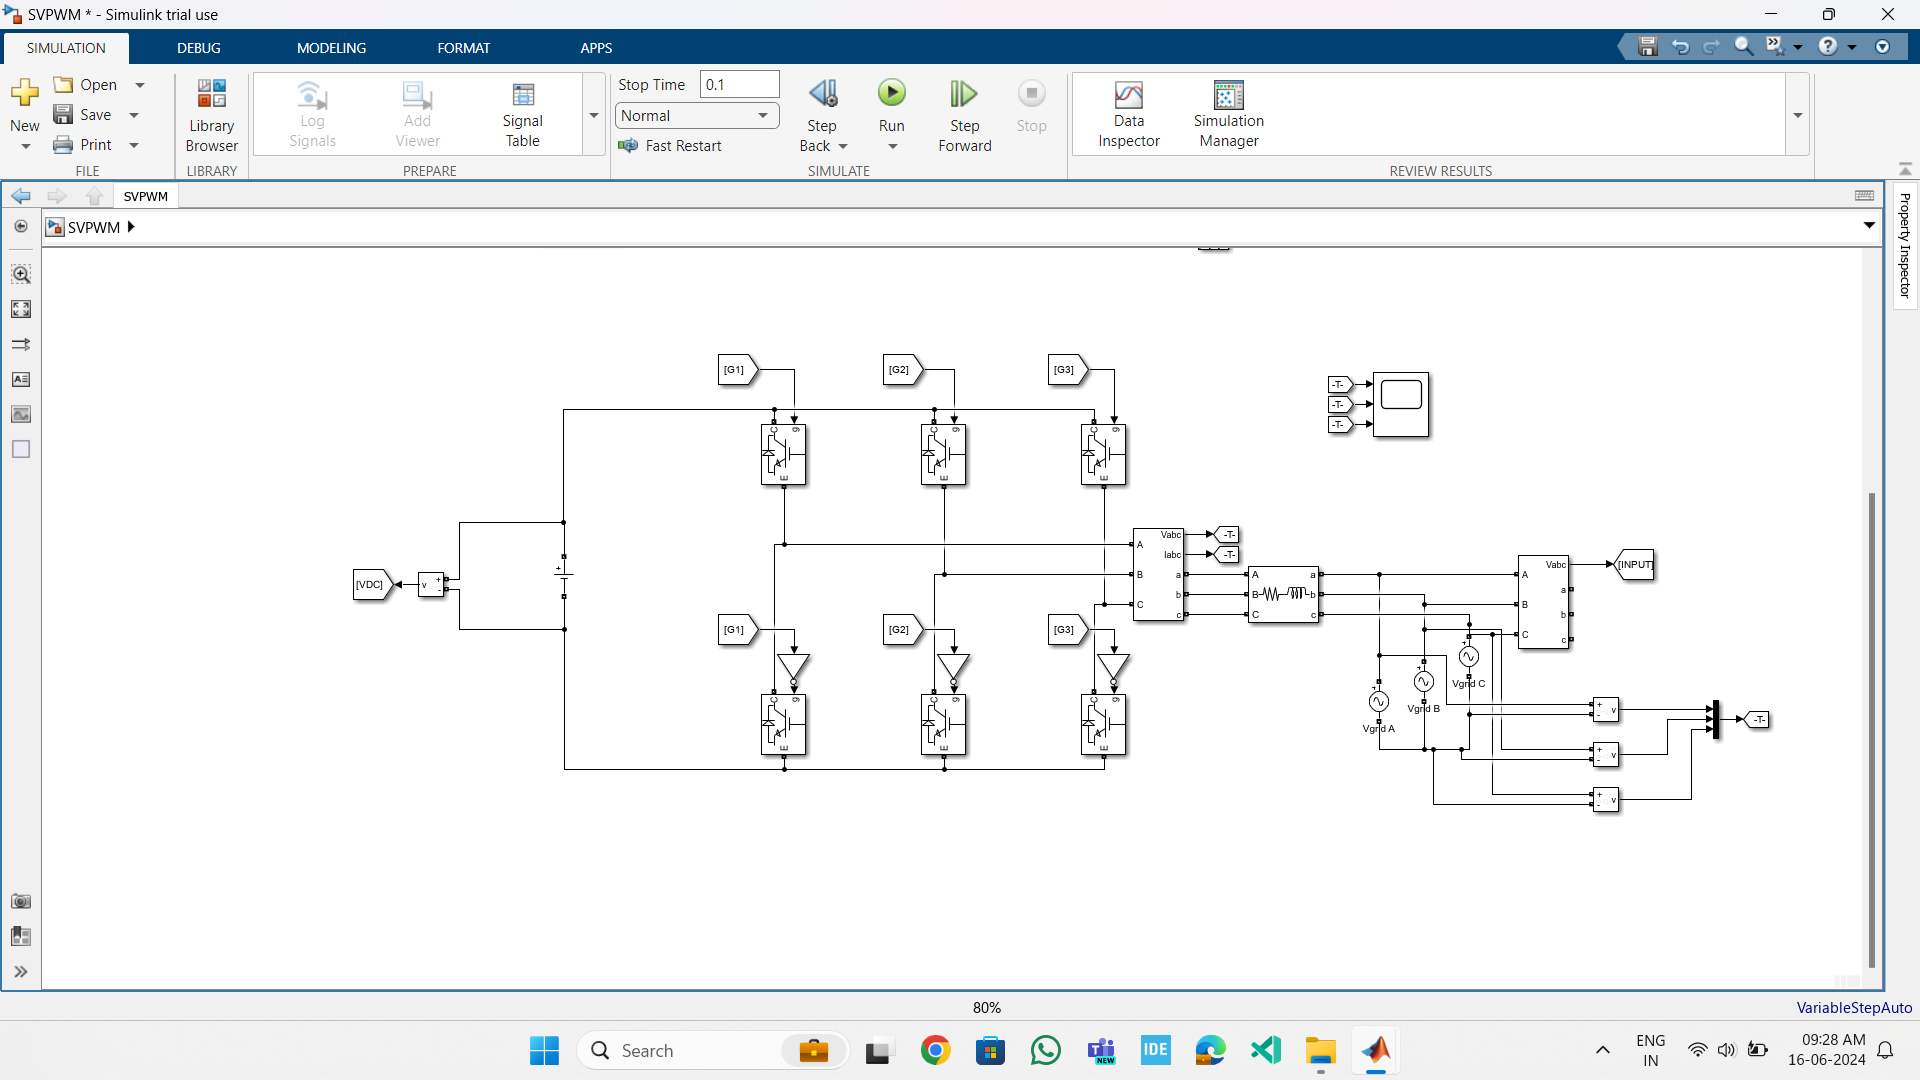
\includegraphics[width=\textwidth]{Power System.png}
    \caption{Power System}
    \label{fig:Power System}
\end{figure}

\subsubsection{Three-Phase AC Source}
The Three-Phase AC Source serves as the input power to the system.It provides
three sinusoidal voltage waveforms with a 120-degree phase difference between
each phase.The amplitude and frequency of the AC source are determined based on
the grid specifications or the application requirements.
\subsubsection{Three-Phase IGBT Bridge}
The Three-Phase IGBT Bridge is the primary power conversion and control element
in the system. It consists of six Insulated Gate Bipolar Transistors (IGBTs)
arranged in a three-phase bridge configuration. The IGBTs are switched in a
complementary manner to modulate the voltage across the load.\\

The IGBT bridge controls the flow of current from the AC source to the load by
switching the IGBTs on and off at precise intervals. This switching action
enables the conversion of AC power from the source to DC power, which can be
further conditioned or inverted as per the requirements of the application.\\

Additionally, the gate timing signals for the IGBTs are generated based on the
control signals calculated by the control system. These gate timing signals
dictate the switching pattern of the IGBTs, ensuring the desired current and
voltage waveforms are maintained for efficient and stable operation of the
power conversion system.

\section{Implementation}
\begin{figure}[h]
    \centering
    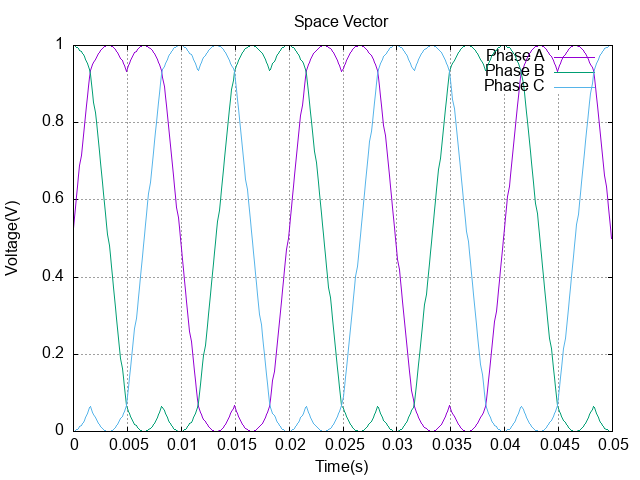
\includegraphics[width=\textwidth]{spacevector.png}
    \caption{Space Vector plotted using GNUPLOT}
    \label{fig:Space Vector Generated using C code}
\end{figure}
After completing the simulation using Simulink/MATLAB to validate
the system design and control strategies, the project transitioned to the
implementation stage on a microcontroller. This phase focused on translating
theoretical concepts into practical application. This section includes the
selection process of the microcontroller, development of essential
transformation functions in C, and the integration of hardware components such
as timers, Direct Memort Access (DMA), and Analog to Digital Converter (ADC)
for accurate system monitoring and control.

\subsection{Microcontroller Selection}
The first step in the implementation phase was choosing an appropriate
microcontroller for the project. After evaluating several options, the
STM32F411 was selected due to its Digital Signal Processing (DSP) and Floating
Point Unit (FPU) capabilities. These features allowed us to run the
Proportional-Integral-Derivative (PID) loop at a high frequency of 10kHz,
providing 200 samples per cycle. This high sampling rate was crucial for
achieving precise control and stability in the system.

\subsection{Implementation of Voltage transform functions}
To handle the transformations required for the control algorithms, I
implemented the Clarke and Park transform functions in C. The process began by
creating an array with synthetic values to simulate the inputs. These values
were then fed into the custom transformation functions. The output was verified
using GNUPLOT to ensure the accuracy of the transformations. This step was
essential to validate the mathematical operations and ensure the functions were
performing as expected.

\subsection{Microcontroller Programming and Testing}
With the transformation functions ready, I proceeded to program the STM32F411
microcontroller. This phase involved a deep dive into various aspects of the
microcontroller, including timers, Direct Memory Access (DMA), and
Analog-to-Digital Converters (ADC).
\begin{itemize}
    \item \textbf{ADC Sampling}: I utilized the ADC to sample the voltage values from the system. This real-time data acquisition was critical for the subsequent control processes.
    \item \textbf{Transformation and Modulation}: The sampled voltage values were processed using the previously developed Clarke and Park transform functions. This step generated the necessary parameters for Space Vector Modulation (SVM).
\end{itemize}
\noindent
The integration of these components allowed for the generation of space vector
modulated waves, essential for controlling the power conversion system
effectively. Each part of this process was meticulously tested to ensure
reliability and accuracy, laying a strong foundation for the successful
deployment of the control system.
\chapter{Details of work}
In this sections I will provide a detailed explanation of each component and
process involved in the implementation phase of the project. Before diving into
the details, it's crucial to establish a foundational understanding of key
concepts that simplify the analysis and control of three-phase circuitry.

\section{Phase-Line Transformation}
\begin{figure}[h]
    \centering
    \begin{subfigure}[b]{0.4\textwidth}
        \centering
        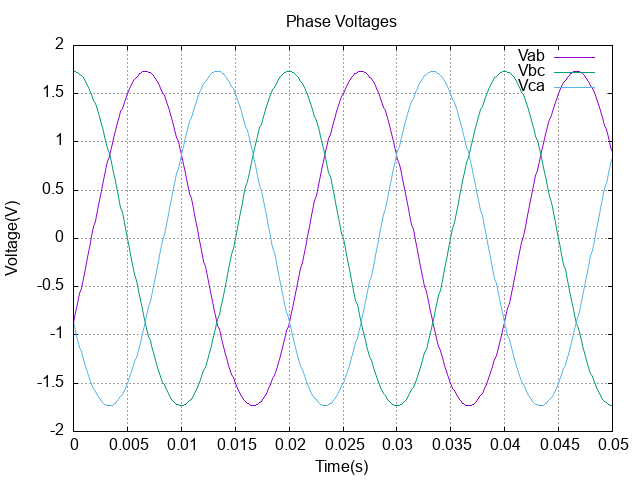
\includegraphics[width=\textwidth]{Phase_Voltages.png}
        \caption{Phase Voltages}
        \label{fig:Phase Voltages}
    \end{subfigure}
    \begin{tikzpicture}
        \node at (0,0) {};
        \draw[->, thick] (0,2.5) -- (1,2.5);
    \end{tikzpicture}
    \begin{subfigure}[b]{0.4\textwidth}
        \centering
        \includegraphics[width=\textwidth]{Line_Voltages.png}
        \caption{Line Voltages}
        \label{fig:Line Voltages}
    \end{subfigure}
\end{figure}

\subsection{Why Measure Phase Voltage?}
In three-phase electrical systems, the measurement of phase voltages becomes
critical due to the unavailability of the neutral point. This unavailability
means that direct measurement of line voltages is not feasible. Phase voltage
refers to the voltage measured across a single component within the three-phase
system, typically between a phase (live) wire and the neutral point. These
measurements are essential because they are the only voltages directly
accessible within the system. Despite this, most voltage transformations and
analyses are conventionally performed on line voltages, which represent the
voltage difference between any two phases in the system. To bridge this gap, it
is imperative to convert the measured phase voltages to line voltages using
precise voltage transformations.

\subsection{Need for Conversion from Phase to Line Voltage}
In a three-phase system, the primary objective is to regulate both the line
current and line voltage accurately. Line voltages, which are the voltages
between any two phases, are crucial for determining the overall performance and
stability of the system. However, since we are limited to measuring phase
voltages, a reliable conversion mechanism is necessary to translate these
measurements into line voltages. This conversion is essential for achieving
accurate control and analysis of the system's electrical parameters. By
converting phase voltages to line voltages, we can apply standard voltage
transformation techniques and ensure that the control strategies and safety
mechanisms are based on accurate and relevant data.

\subsection{Why Simply Dividing by the Square Root of 3 is Insufficient}
A common misconception is that dividing the measured phase voltage by the
square root of 3 will yield the correct line voltage. This approach is based on
the RMS (Root Mean Square) values and is only accurate for calculating the
magnitude of the line voltage under steady-state, balanced conditions. The
relationship \(phase\ voltage = \sqrt{3} \times line\ voltage\) holds true only
for the RMS values of sinusoidal voltages in a perfectly balanced system.
However, for dynamic applications, such as those involving digital signal
processing (DSP), we require instantaneous line voltages rather than just RMS
magnitudes.\\

Instantaneous voltages account for the real-time variations and phase
differences that occur in practical systems. Therefore, a more robust method is
necessary to obtain these instantaneous values accurately. To address this
requirement, we use a transformation matrix that accurately converts the phase
voltages to line voltages. The transformation matrix employed is:

\begin{equation*}
    T_{line} =
    \begin{bmatrix}
        \frac{2}{3}  & \frac{1}{3}  & 0 \\
        \frac{-1}{3} & \frac{1}{3}  & 0 \\
        \frac{-1}{3} & \frac{-2}{3} & 0
    \end{bmatrix}
\end{equation*}

This matrix provides a precise method to convert the three measured phase
voltages into their corresponding line voltages, ensuring that the
instantaneous values required for DSP and other real-time control applications
are accurately obtained. This approach eliminates the inaccuracies associated
with simple RMS-based conversion and allows for a more accurate representation
of the system's electrical characteristics in real-time operations.

\subsection{Derivation of the Transformations}
For this conversion, we need to define a matrix, so let's look at the
derivation for such a matrix.

Let \( V_a, V_b, V_c \) be the phase voltages given by:
\[
    V_a = \sin(\omega t)
\]
\[
    V_b = \sin(\omega t - 120^\circ)
\]
\[
    V_c = \sin(\omega t + 120^\circ)
\]

The line voltages \( V_{ab}, V_{bc}, V_{ca} \) are given by:
\[
    V_{ab} = V_a - V_b
\]
\[
    V_{bc} = V_b - V_c
\]
\[
    V_{ca} = V_c - V_a
\]

Also, we know that:
\[
    V_a + V_b + V_c = 0
\]

Let us assume two matrices: \( P \), representing phase voltages, and \( L \),
representing line voltages:
\[
    P = \begin{bmatrix}
        V_a \\
        V_b \\
        V_c \\
    \end{bmatrix}
\]
\[
    L = \begin{bmatrix}
        V_{ab} \\
        V_{bc} \\
        V_{ca} \\
    \end{bmatrix}
\]

Let \( T \) be a transformation matrix from \( P \) to \( L \):
\[
    L = T \cdot P
\]

We can define \( T \) as:
\[
    T = \begin{bmatrix}
        1  & -1 & 0  \\
        0  & 1  & -1 \\
        -1 & 0  & 1  \\
    \end{bmatrix}
\]

Since the inverse of \( T \) does not exist, we redefine it as:
\[
    \begin{bmatrix}
        V_{ab} \\
        V_{bc} \\
        V_{ca} \\
        0      \\
    \end{bmatrix} = \begin{bmatrix}
        1  & -1 & 0  & 1 \\
        0  & 1  & -1 & 1 \\
        -1 & 0  & 1  & 1 \\
        1  & 1  & 1  & 1 \\
    \end{bmatrix} \begin{bmatrix}
        V_a \\
        V_b \\
        V_c \\
        0   \\
    \end{bmatrix}
\]

Taking the inverse of \( T \):
\[
    T^{-1} = \begin{bmatrix}
        \frac{2}{9}  & -\frac{1}{9} & -\frac{4}{9} & \frac{1}{3} \\
        -\frac{4}{9} & \frac{2}{9}  & -\frac{1}{9} & \frac{1}{3} \\
        -\frac{1}{9} & -\frac{4}{9} & \frac{2}{9}  & \frac{1}{3} \\
        \frac{1}{3}  & \frac{1}{3}  & \frac{1}{3}  & 0           \\
    \end{bmatrix}
\]

Solving the matrix:
\[
    V_a = \frac{2}{9}V_{ab} - \frac{1}{9}V_{bc} - \frac{4}{9}V_{ca}
\]
\[
    V_b = -\frac{4}{9}V_{ab} + \frac{2}{9}V_{bc} - \frac{1}{9}V_{ca}
\]
\[
    V_c = -\frac{1}{9}V_{ab} - \frac{4}{9}V_{bc} + \frac{2}{9}V_{ca}
\]

We also know that \( V_{ab} + V_{bc} + V_{ca} = 0 \), so:
\[
    V_{ca} = -V_{ab} - V_{bc}
\]

Thus:
\[
    V_a = \frac{2}{3}V_{ab} + \frac{1}{3}V_{bc}
\]
\[
    V_b = -\frac{1}{3}V_{ab} + \frac{1}{3}V_{bc}
\]
\[
    V_c = -\frac{1}{3}V_{ab} - \frac{2}{3}V_{bc}
\]

So, we can define the transformation matrix as:
\[
    T_{line}^{-1} = \begin{bmatrix}
        \frac{2}{9}  & -\frac{1}{9} & -\frac{4}{9} \\
        -\frac{4}{9} & \frac{2}{9}  & -\frac{1}{9} \\
        -\frac{1}{9} & -\frac{4}{9} & \frac{2}{9}  \\
    \end{bmatrix}
\]

\section{Clarke transform}
The alpha-beta transform, also known as the Clarke transform, is a fundamental
mathematical tool used to simplify the analysis of three-phase electric
machines. It is named after Edith Clarke, who published papers in 1937 and 1938
introducing modified calculation methods for handling unbalanced three-phase
problems~\cite{E. Clarke}.

\subsection{What is Clarke Transform?}
\begin{figure}[ht]
    \centering
    \resizebox{0.4\linewidth}{!}{
        \begin{tikzpicture}[auto, node distance=2cm, >=Latex]
            % Define the origin
            \coordinate (O) at (0,0);

            % Define the vectors
            \coordinate (A) at ({3*cos(0)},{3*sin(0)});
            \coordinate (B) at ({3*cos(120)},{3*sin(120)});
            \coordinate (C) at ({3*cos(240)},{3*sin(240)});
            \coordinate (alpha) at ({3.8*cos(0)},{3.8*sin(0)});
            \coordinate (beta) at ({3.8*cos(90)},{3.8*sin(90)});

            % Draw the main axes
            \draw[->] (O) -- (B) node[above] {$B$-axis};
            \draw[->] (O) -- (C) node[below] {$C$-axis};
            \draw[->] (O) -- (A) node[below] {$A$-axis};

            % Draw the Clarke axes
            \draw[thick, ->] (O) -- (alpha) node[below right] {$\alpha$-axis};
            \draw[thick, ->] (O) -- (beta)  node[above right] {$\beta$-axis};

            % Draw the angular velocity indication
            % \draw[->] (1,1.5) arc[start angle=60, end angle=90, radius=1.5cm];
            % \node at (1.5,2) {$\omega=0$};

        \end{tikzpicture}
    }
    \caption{Clarke Frame of reference}
    \label{fig:Clarke Frame of reference}
\end{figure}

E. Clarke developed the method for transforming stationary circuits into a
stationary reference frame. In Clarke’s transformation, the two-phase
stationary variables are represented as $\alpha$ and $\beta$, with the
$\alpha$-axis and $\beta$-axis being orthogonal to each other~\cite{DSP-Based
    Electromechanical Motion Control}.This transformation simplifies the analysis
of three-phase electrical systems by projecting the original quantities onto a
stationary reference frame. It decomposes the three-phase variables into two
orthogonal components: alpha ($\alpha$) and beta ($\beta$), which are aligned
with the stationary reference axes, called the Clarke reference frame. The
transform matrix is given by:
\begin{equation*}
    T_{\alpha\beta0} = \frac{2}{3}
    \begin{bmatrix}
        1 & -\frac{1}{2}       & -\frac{1}{2}       \\
        0 & \frac{\sqrt{3}}{2} & \frac{\sqrt{3}}{2} \\
        1 & 1                  & 1
    \end{bmatrix}
\end{equation*}


\subsection{Derivation of the Clarke Transform Matrix}

\begin{figure}[h]
    \centering
    \begin{subfigure}[b]{0.5\textwidth}
        \centering
        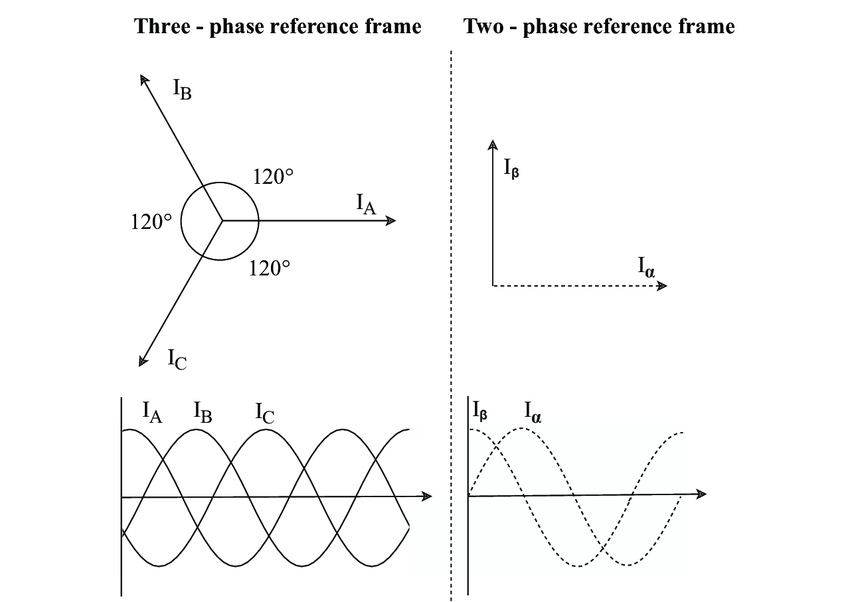
\includegraphics[width=\textwidth]{Clarke-transformation-coordinates.png}
        \caption{Clarke transformation}
        \label{fig:Clarke transformation}
    \end{subfigure}%
    \begin{subfigure}[b]{0.5\textwidth}
        \centering
        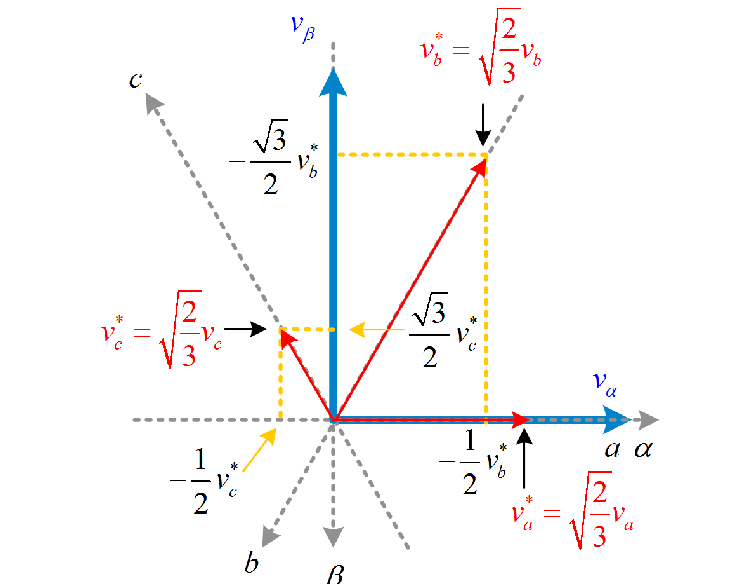
\includegraphics[width=\textwidth]{clarkederivation.png}
        \caption{Clarke transformation Derivation}
        \label{fig:Clarke transformation Derivation}
    \end{subfigure}
    \caption{Clarke transformation and its derivation}
    \label{fig:combined_Clarke}
\end{figure}


To derive the Clarke transformation, we resolve the three-phase quantities \(
V_a, V_b, V_c \) along the \(\alpha\) and \(\beta\) axes. The transformed
quantities \( V_\alpha \) and \( V_\beta \) are simplified according to Figure
\ref{fig:Clarke transformation Derivation}. The normalization term \(
\frac{2}{3} \) ensures that the magnitudes of the quantities in the Clarke
frame match those of the three-phase frame.

\begin{equation*}
    V_\alpha = \frac{2}{3}(V_a - \frac{1}{2} V_b - \frac{1}{2} V_c)
\end{equation*}
\begin{equation*}
    V_\beta = \frac{2}{3}(\frac{\sqrt{3}}{2} V_b - \frac{\sqrt{3}}{2} V_c)
\end{equation*}

\noindent
Converting this to matrix form, we get:
\begin{equation*}
    \begin{bmatrix}
        V_\alpha \\
        V_\beta  \\
        V_0
    \end{bmatrix}
    =\frac{2}{3}
    \begin{bmatrix}
        1 & -\frac{1}{2}       & -\frac{1}{2}       \\
        0 & \frac{\sqrt{3}}{2} & \frac{\sqrt{3}}{2} \\
        1 & 1                  & 1
    \end{bmatrix}
    \begin{bmatrix}
        V_a \\
        V_b \\
        V_c
    \end{bmatrix}
\end{equation*}
\noindent
or we can write it as:
\begin{equation*}
    V_{\alpha\beta0} = T_{\alpha\beta0} V_{abc}
\end{equation*}

\noindent
Where,
\begin{equation*}
    V_{\alpha\beta0} = \begin{bmatrix}
        V_\alpha \\
        V_\beta  \\
        V_0
    \end{bmatrix}
\end{equation*}
\begin{equation*}
    V_{abc} = \begin{bmatrix}
        V_a \\
        V_b \\
        V_c
    \end{bmatrix}
\end{equation*}
\begin{equation*}
    T_{\alpha\beta0} = \frac{2}{3}
    \begin{bmatrix}
        1 & -\frac{1}{2}       & -\frac{1}{2}       \\
        0 & \frac{\sqrt{3}}{2} & \frac{\sqrt{3}}{2} \\
        1 & 1                  & 1
    \end{bmatrix}
\end{equation*}

\noindent
For a balanced three-phase system where \( V_a + V_b + V_c = 0 \), the equations simplify to:
\begin{equation*}
    V_\alpha = V_a
\end{equation*}
\begin{equation*}
    V_\beta = \frac{2}{\sqrt{3}} (V_a + 2 V_b)
\end{equation*}
\begin{equation*}
    V_0 = 0
\end{equation*}
\section{Park transform}
The Park transform, also known as the \( dq \) transformation, is another
fundamental mathematical tool used in the analysis of three-phase electric
machines.In the late 1920s, R.H. Park\cite{R. H. Park} introduced a new
approach to electric machine analysis. He formulated a change of variables
which replaced variables such as voltages, currents, and flux linkages
associated with fictitious windings rotating with the rotor. He referred the
stator and rotor variables to a reference frame fixed on the rotor. From the
rotor point of view, all the variables can be observed as constant values
\subsection{What is Park Transform?}
\begin{figure}[ht]
    \centering
    \resizebox{0.5\linewidth}{!}{
        \begin{tikzpicture}
            % Draw the coordinate axes
            \draw[->] (0,0) -- (5,0) node[anchor=north] {$\alpha$};
            \draw[->] (0,0) -- (0,5) node[anchor=east] {$\beta$};
            \draw[->, thick] (0,0) -- (-4,3) node[anchor=east] {$q$};
            \draw[->, thick] (0,0) -- (3,4) node[anchor=west] {$d$};

            % Draw the angle theta
            \draw (1,0) arc (0:53:1);
            \node at (1.2,0.6) {$\theta$};

            % Draw the omega arc
            \draw[->] (2,2.67) arc (53:90:1);
            \node at (2.3,3.5) {$\omega$};

            % Draw the right angle symbol
            \draw (0.3,0) -- (0.3,0.3) -- (0,0.3);
        \end{tikzpicture}
    }
    \caption{Park Frame of reference}
    \label{Park Frame of reference}
\end{figure}
The Park transform shifts the perspective from the traditional stationary
reference frame to a rotating reference frame that moves with the rotor. This
transformation effectively decouples the complex interactions between variables
such as voltages, currents, and flux linkages that occur in three-phase
systems. By aligning with the rotor's magnetic field, the transform separates
these variables into two orthogonal components: \( d \) (direct) and \( q \)
(quadrature). Figure:\ref{fig:Park Transform}\\

In practical terms, within the \( dq \) frame, \( d \) represents the component
aligned with the rotor flux (direct axis), while \( q \) represents the
component perpendicular to the rotor flux (quadrature axis). This separation
facilitates independent control of the torque-producing and magnetizing
currents in field-oriented control strategies, essential for optimizing the
performance of electric machines.
\begin{figure}[h]
    \centering
    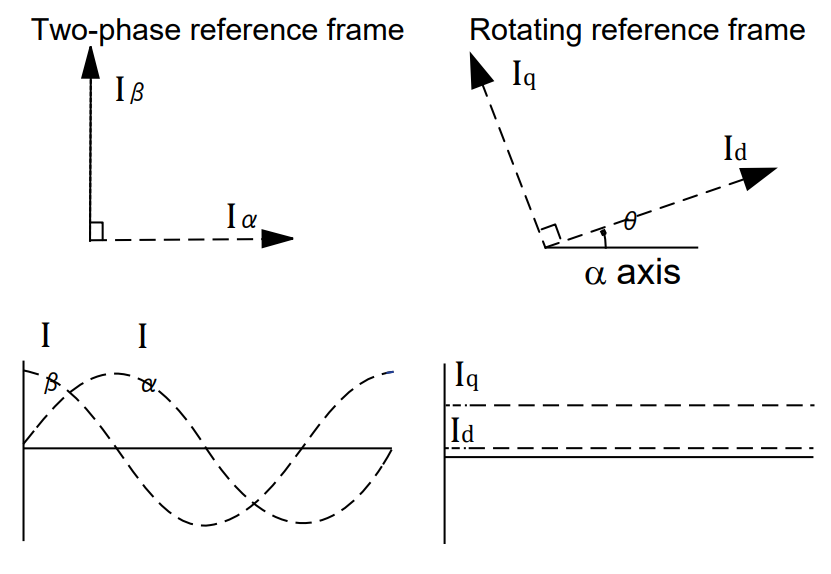
\includegraphics[width=0.6\textwidth]{park-clarke.png}
    \caption{Park Transform}
    \label{fig:Park Transform}
\end{figure}

To derive the Park transformation matrix, we first define the transformation
angle \( \theta \), which corresponds to the rotor angle. By applying an axis
rotation and rotating the Clarke frame by \( \theta \), we obtain the
transformation matrix \( T_{dq0} \).

\begin{equation*}
    T_{dq0} =
    \begin{bmatrix}
        \cos \theta & -\sin \theta & 0 \\
        \sin \theta & \cos \theta  & 0 \\
        0           & 0            & 1
    \end{bmatrix}
\end{equation*}

\subsection{Derivation of the Park Transform Matrix}

\noindent
Where \( \theta \) is the electrical angle of the rotor position.
\noindent
The Park transform equations for transforming the three-phase quantities \(
V_\alpha, V_\beta, V_0 \) to the \( dq \) frame are:

\begin{equation*}
    V_d = V_\alpha \cos \theta + V_\beta \sin \theta
\end{equation*}
\begin{equation*}
    V_q = -V_\alpha \sin \theta + V_\beta \cos \theta
\end{equation*}
\begin{equation*}
    V_0 = V_0
\end{equation*}
\noindent
Converting these equations into matrix form, we get:

\begin{equation*}
    \begin{bmatrix}
        V_d \\
        V_q \\
        V_0
    \end{bmatrix}
    =
    \begin{bmatrix}
        \cos \theta & -\sin \theta & 0 \\
        \sin \theta & \cos \theta  & 0 \\
        0           & 0            & 1
    \end{bmatrix}
    \begin{bmatrix}
        V_\alpha \\
        V_\beta  \\
        V_0
    \end{bmatrix}
\end{equation*}
\noindent
or in the shorthand notation:
\begin{equation*}
    V_{dq0} = T_{dq0} V_{\alpha\beta0}
\end{equation*}
\noindent
Where:
\begin{equation*}
    V_{dq0} = \begin{bmatrix}
        V_d \\
        V_q \\
        V_0
    \end{bmatrix}
\end{equation*}
\begin{equation*}
    V_{\alpha\beta0} = \begin{bmatrix}
        V_\alpha \\
        V_\beta  \\
        V_0
    \end{bmatrix}
\end{equation*}
\begin{equation*}
    T_{dq0} =
    \begin{bmatrix}
        \cos \theta & -\sin \theta & 0 \\
        \sin \theta & \cos \theta  & 0 \\
        0           & 0            & 1
    \end{bmatrix}
\end{equation*}

\section{PID Controller}
The Proportional Integral Derivative (PID) Controller\cite{pid-wikipedia} is
the most widely used control technique in industry. The popularity of PID
Controller because of their robust performance in a wide range of operating
condition and its simple functionality. Industrial processes are subjected to
variation in parameters and parameters perturbations.

\begin{figure}[ht]
    \centering
    \resizebox{\linewidth}{!}{
        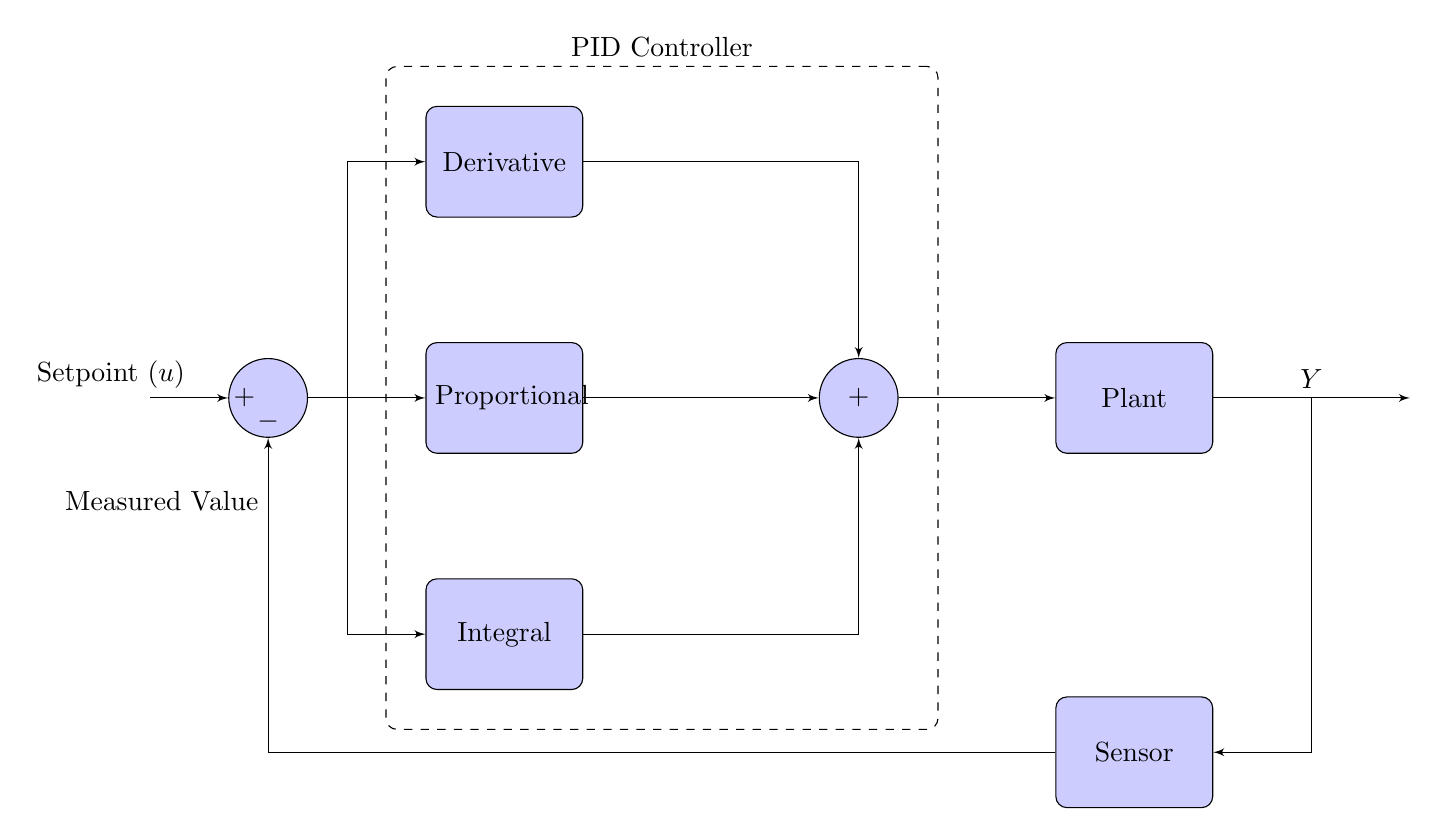
\begin{tikzpicture}[auto, node distance=2cm,>=latex']
            % Nodes
            \node [input, name=input] {};
            \node [sum, right of=input] (sum) {};
            \node at ([xshift=-0.3cm]sum.center) {$+$};
            \node at ([yshift=-0.3cm]sum.center) {$-$};

            \node [block, right of=sum, node distance=3cm] (P) {Proportional};
            \node [block, below of=P, node distance=3cm] (I) {Integral};
            \node [block, above of=P, node distance=3cm] (D) {Derivative};

            \node [sum, right of=P, node distance=4.5cm] (sumPID) {$+$};
            \node [block, right of=sumPID, node distance=3.5cm] (plant) {Plant};
            \node [output, right of=plant, node distance=3.5cm] (output) {};
            \node [block, below of=plant, node distance=4.5cm] (sensor) {Sensor};

            % PID Controller dashed box
            \node [pidblock, fit=(P) (I) (D) (sumPID), label=above:PID Controller] {};

            % Connections
            \draw [draw,->] (input) -- node[name=setpoint,pos=-0.5] {Setpoint ($u$)} (sum);
            \draw [->] (sum.east) -- ++(0.5,0) |- (P.west);
            \draw [->] (sum.east) -- ++(0.5,0) |- (I.west);
            \draw [->] (sum.east) -- ++(0.5,0) |- (D.west);

            \draw [->] (P) -- (sumPID);
            \draw [->] (I) -| (sumPID);
            \draw [->] (D) -| (sumPID);

            \draw [->] (sumPID) -- (plant);
            \draw [->] (plant) -- node [name=measure] {$Y$} (output);
            \draw [->] (measure) |- (sensor);
            \draw [->] (sensor) -| node[pos=0.9] {Measured Value} (sum); % Adjusted position here
        \end{tikzpicture}
    }
    \caption{PID Controller Diagram.}
    \label{fig:pid_diagram}
\end{figure}

\subsection{What is PID Controller?}
A PID Controller consists of a controlled system known as the Plant and a
Controller designed to manage the overall system behavior. The transfer
function of the PID Controller in the S-domain is given by:
\begin{equation*}
    K_p + \frac{K_i}{S}+K_d S
\end{equation*}

Where $K_p$ is the proportional gain, $K_i$ is the integral gain, and $K_d$ is
the derivative gain. The error ($e$) is the difference between the desired
reference value ($R$) and the actual output ($Y$). The controller processes
this error signal, computing its derivative and integral. The signal sent to
the actuator ($u$) is:
\begin{equation*}
    u(t) = K_p e(t) + K_i \int_{0}^{t} e(\tau) \, d\tau + K_d \frac{de(t)}{dt}
\end{equation*}

This output signal ($u$) is sent to the plant, resulting in a new output ($Y$).
This output is then fed back to compute a new error ($e$). The PID Controller
continuously processes the new error signal, calculating its derivative and
integral in an ongoing loop.

\subsection{Feedforward Control}

While PID controllers are effective at correcting errors based on feedback from
the process variable (Process Variable), they can be enhanced by incorporating
Feedforward Control. Feedforward Control is a proactive approach that
anticipates disturbances and preemptively adjusts the controller output to
minimize their effects on the Process Variable.

\subsubsection{Why Use Feedforward Control?}

In industrial processes, disturbances such as changes in feed flow rates,
variations in raw material quality, or environmental factors can significantly
impact the Process Variable. These disturbances are often unpredictable and can
lead to deviations from the setpoint, requiring the PID controller to react and
correct the error. However, by the time the disturbance affects the Process
Variable, some amount of error may have already occurred.\\

Feedforward Control\cite{feedforward-wikipedia} addresses this issue by using a
model or direct measurement of the disturbance to predict its effect on the
Process Variable. This prediction is used to generate a feedforward signal that
is added to the PID controller's output. By doing so, the controller
compensates for the disturbance before it affects the Process Variable, thereby
reducing the error and improving the response time.

\subsubsection{Types of Feedforward Control}

There are two main types of Feedforward Control:

\begin{enumerate}
    \begin{figure}[ht]
        \centering
        \resizebox{\linewidth}{!}{
            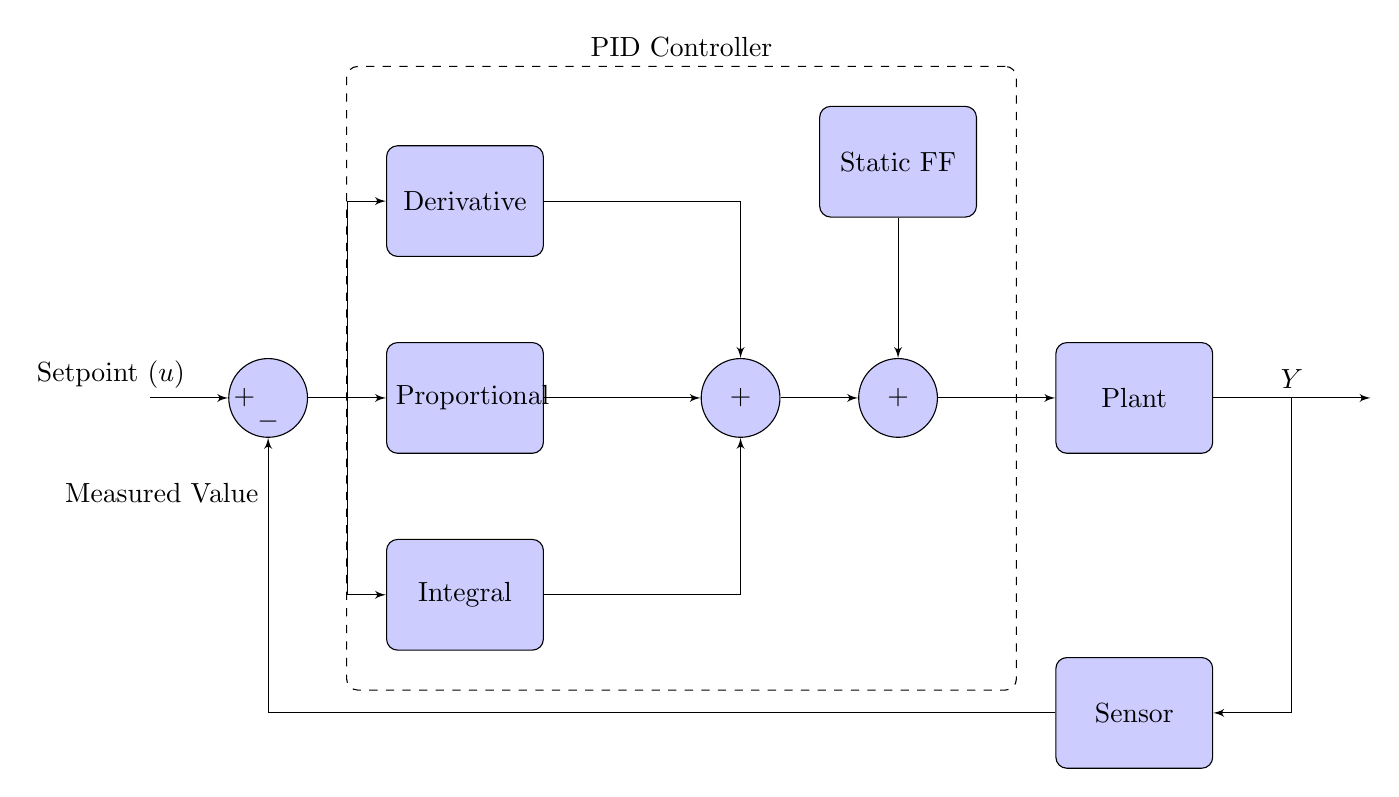
\begin{tikzpicture}[auto, node distance=2cm,>=latex']
                % Nodes
                \node [input, name=input] {};
                \node [sum, right of=input] (sum) {};
                \node at ([xshift=-0.3cm]sum.center) {$+$};
                \node at ([yshift=-0.3cm]sum.center) {$-$};

                \node [block, right of=sum, node distance=2.5cm] (P) {Proportional};
                \node [block, below of=P, node distance=2.5cm] (I) {Integral};
                \node [block, above of=P, node distance=2.5cm] (D) {Derivative};

                \node [sum, right of=P, node distance=3.5cm] (sumPID) {$+$};
                \node [sum, right of=sumPID, node distance=2cm] (sumFF) {$+$};
                \node [block, right of=sumFF, node distance=3cm] (plant) {Plant};
                \node [output, right of=plant, node distance=3cm] (output) {};
                \node [block, below of=plant, node distance=4cm] (sensor) {Sensor};

                \node [block, above of=sumFF, node distance=3cm] (FF) {Static FF};

                % PID Controller dashed box
                \node [pidblock, fit=(P) (I) (D) (sumPID) (FF), label=above:PID Controller] {};

                % Connections
                \draw [draw,->] (input) -- node[name=setpoint,pos=-0.5] {Setpoint ($u$)} (sum);
                \draw [->] (sum.east) -- ++(0.5,0) |- (P.west);
                \draw [->] (sum.east) -- ++(0.5,0) |- (I.west);
                \draw [->] (sum.east) -- ++(0.5,0) |- (D.west);

                \draw [->] (P) -- (sumPID);
                \draw [->] (I) -| (sumPID);
                \draw [->] (D) -| (sumPID);

                \draw [->] (sumPID) -- node {} (sumFF);
                \draw [->] (sumFF) -- node {} (plant);
                \draw [->] (plant) -- node [name=measure] {$Y$} (output);
                \draw [->] (measure) |- (sensor);
                \draw [->] (sensor) -| node[pos=0.9] {Measured Value} (sum); % Adjusted position here

                % Static FF connection
                \draw [->] (FF) -- (sumFF);

            \end{tikzpicture}
        }
        \caption{PID Controller and Static Feedforward Control.}
        \label{fig:_pid_ff}
    \end{figure}
    \item \textbf{Static Feedforward Control}: This type calculates a steady-state gain based on the relationship between the disturbance variable and the Process Variable. The calculated gain is then added directly to the controller output. While effective for steady disturbances, it does not account for dynamic changes in the process.
          \begin{figure}[ht]
              \centering
              \resizebox{\linewidth}{!}{
                  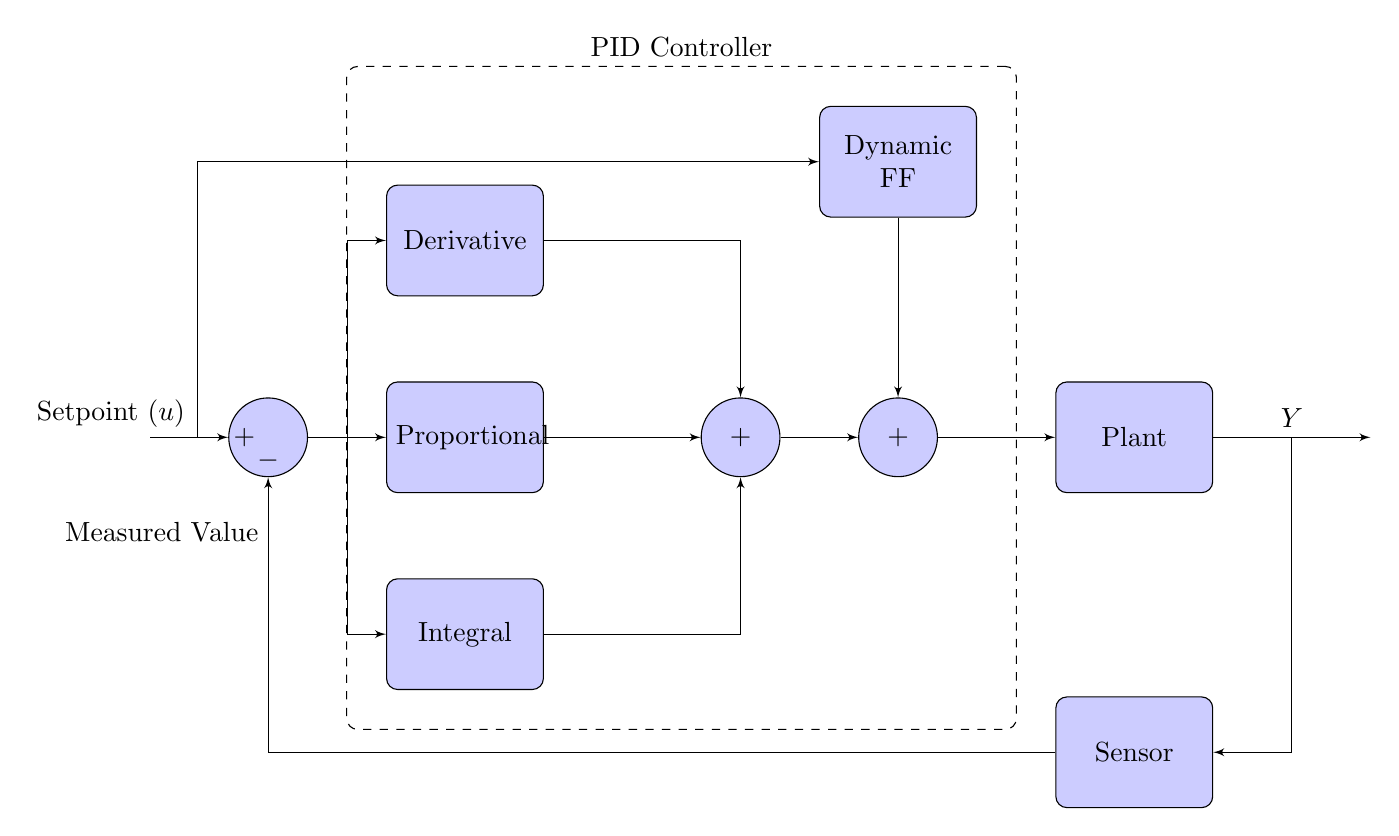
\begin{tikzpicture}[auto, node distance=2cm,>=latex']
                      % Nodes
                      \node [input, name=input] {};
                      \node [sum, right of=input] (sum) {};
                      \node at ([xshift=-0.3cm]sum.center) {$+$};
                      \node at ([yshift=-0.3cm]sum.center) {$-$};

                      \node [block, right of=sum, node distance=2.5cm] (P) {Proportional};
                      \node [block, below of=P, node distance=2.5cm] (I) {Integral};
                      \node [block, above of=P, node distance=2.5cm] (D) {Derivative};

                      \node [sum, right of=P, node distance=3.5cm] (sumPID) {$+$};
                      \node [sum, right of=sumPID, node distance=2cm] (sumFF) {$+$};
                      \node [block, right of=sumFF, node distance=3cm] (plant) {Plant};
                      \node [output, right of=plant, node distance=3cm] (output) {};
                      \node [block, below of=plant, node distance=4cm] (sensor) {Sensor};

                      \node [block, above of=sumFF, node distance=3.5cm] (FF) {Dynamic FF};

                      % PID Controller dashed box
                      \node [pidblock, fit=(P) (I) (D) (sumPID) (FF), label=above:PID Controller] {};

                      % Connections
                      \draw [draw,->] (input) -- node[name=setpoint,pos=-0.5] {Setpoint ($u$)} (sum);
                      \draw [->] (sum.east) -- ++(0.5,0) |- (P.west);
                      \draw [->] (sum.east) -- ++(0.5,0) |- (I.west);
                      \draw [->] (sum.east) -- ++(0.5,0) |- (D.west);

                      \draw [->] (P) -- (sumPID);
                      \draw [->] (I) -| (sumPID);
                      \draw [->] (D) -| (sumPID);

                      \draw [->] (sumPID) -- node {} (sumFF);
                      \draw [->] (sumFF) -- node {} (plant);
                      \draw [->] (plant) -- node [name=measure] {$Y$} (output);
                      \draw [->] (measure) |- (sensor);
                      \draw [->] (sensor) -| node[pos=0.9] {Measured Value} (sum); % Adjusted position here

                      % Dynamic FF connection
                      \draw [->] (input) -- ++(0.6,0) |-  (FF);
                      \draw [->] (FF) -- (sumFF);

                  \end{tikzpicture}
              }
              \caption{PID Controller and Dynamic Feedforward Control.}
              \label{fig:_pid_ff_dyn}
          \end{figure}
    \item \textbf{Dynamic Feedforward Control}: Dynamic Feedforward Control considers the dynamic response of the process to disturbances. It incorporates the time constant and dynamics of the disturbance to provide a more accurate compensation. This approach requires a model of the process dynamics or real-time measurement of the disturbance.
\end{enumerate}

\subsubsection{Benefits of Feedforward Control}

\begin{itemize}
    \item \textbf{Improved Disturbance Rejection}: By preemptively adjusting the controller output, Feedforward Control can significantly reduce deviations from the setpoint caused by disturbances.

    \item \textbf{Enhanced Stability}: Minimizing the impact of disturbances helps maintain stability in the control loop, reducing oscillations and improving overall system performance.

    \item \textbf{Efficiency}: Reducing the need for corrective action by the PID controller can extend equipment life and improve process efficiency.
\end{itemize}

In conclusion, while PID controllers excel in maintaining setpoints based on
feedback from the Process Variable, integrating Feedforward Control can enhance
their performance by mitigating the effects of disturbances. By combining both
feedback and feedforward strategies, industrial processes can achieve more
robust and responsive control.

\subsection{Zeigler-Nichols method}
The Ziegler--Nichols tuning method is a heuristic method for tuning a PID
controller, developed by John G. Ziegler and Nathaniel B. Nichols
\cite{ziegler-nichols}. It involves setting the integral (\( T_i \)) and
derivative (\( T_d \)) gains to zero and gradually increasing the proportional
gain (\( K_p \)) until stable oscillations occur at the ultimate gain (\( K_u
\)) and oscillation period (\( T_u \)). The parameters for different types of
controllers are set based on these values, as shown in Table
\ref{tab:ziegler-nichols}.

\begin{table}[ht]
    \centering
    \caption{Ziegler--Nichols Method Parameters for PID Controllers}
    \label{tab:ziegler-nichols}
    \begin{tabular}{|l|c|c|c|c|c|}
        \hline
        Control Type         & \( K_p \)                  & \( T_i \)                  & \( T_d \)                   & \( K_i \)                              & \( K_d \)                      \\
        \hline
        P                    & \( 0.5 K_u \)              & -                          & -                           & -                                      & -                              \\
        PI                   & \( 0.45 K_u \)             & \( 0.8 \overline{3} T_u \) & -                           & \( 0.54 \frac{K_u}{T_u} \)             & -                              \\
        PD                   & \( 0.8 K_u \)              & -                          & \( 0.125 T_u \)             & -                                      & \( 0.10 \frac{K_u}{T_u} \)     \\
        Classic PID          & \( 0.6 K_u \)              & \( 0.5 T_u \)              & \( 0.125 T_u \)             & \( 1.2 \frac{K_u}{T_u} \)              & \( 0.075 \frac{K_u}{T_u} \)    \\
        Pessen Integral Rule & \( 0.7 K_u \)              & \( 0.4 T_u \)              & \( 0.15 T_u \)              & \( 1.75 \frac{K_u}{T_u} \)             & \( 0.105 \frac{K_u}{T_u} \)    \\
        Some Overshoot       & \( 0.3 \overline{3} K_u \) & \( 0.5 T_u \)              & \( 0.3 \overline{3}{T_u} \) & \( 0.6 \overline{6} \frac{K_u}{T_u} \) & \( 0.1 \overline{1} K_u T_u \) \\
        No Overshoot         & \( 0.2 K_u \)              & \( 0.5 T_u \)              & \( 0.3 \overline{3}{T_u} \) & \( 0.4 \frac{K_u}{T_u} \)              & \( 0.6 \overline{6} K_u T_u \) \\
        \hline
    \end{tabular}
\end{table}

The ultimate gain \( K_u \) is defined as \( 1/M \), where \( M \) is the
amplitude ratio. The parameters \( K_i \) and \( K_d \) are derived from \( K_p
\), \( T_i \), and \( T_d \).
\section{Phase Lock Loop (PLL)}
\begin{figure}[ht]
    \centering
    \resizebox{\linewidth}{!}{
        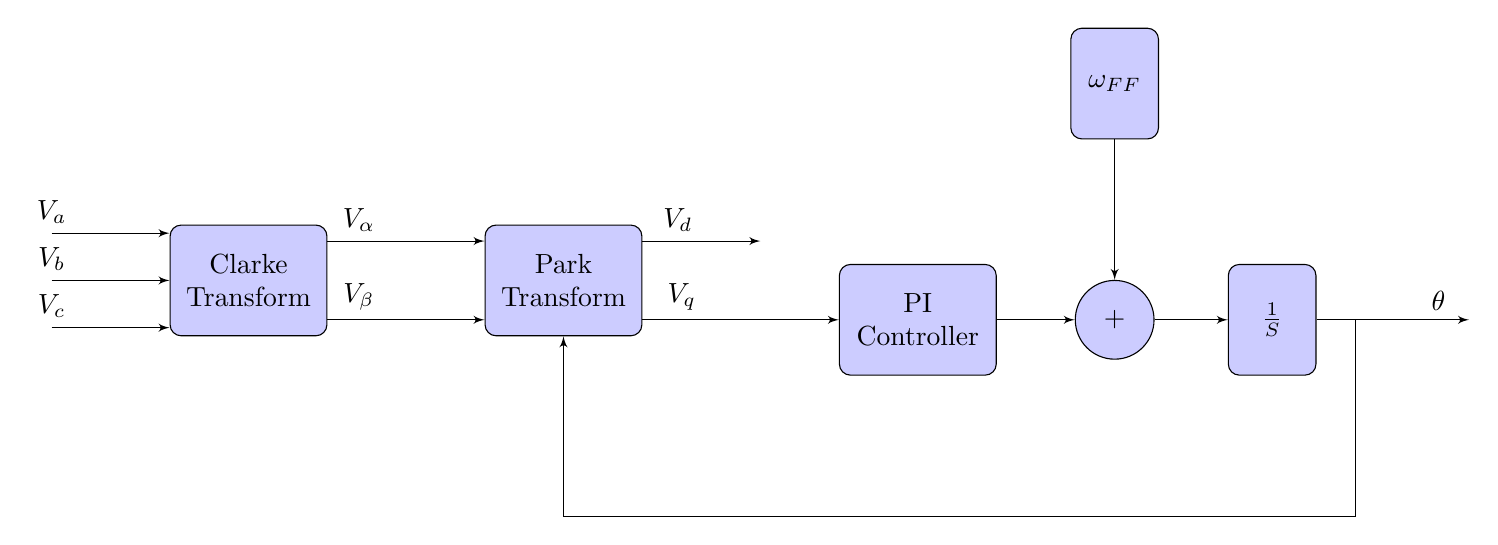
\begin{tikzpicture}[auto, node distance=2cm,>=latex']
            % Nodes
            \node [input] (Vb) {7};
            \node [input, below of=Vb, node distance=0.6cm] (Vc) {};
            \node [input, above of=Vb, node distance=0.6cm] (Va) {};
            \node [block, right of=Vb, node distance=2.5cm] (clarke) {Clarke Transform};
            \node [block, right of=clarke, node distance =4cm] (park) {Park Transform};
            \node [block, right of=park, node distance =4.5cm,yshift=-0.5cm] (pid) {PI \\ Controller};
            \node [output, right of=park, node distance=2.5cm,yshift=0.5cm] (output_Vq) {};
            \node [sum, right of=pid,node distance=2.5cm](sumff){$+$};
            \node [block, above of=sumff,node distance=3cm, text width=2.5em](ff){$\omega_{FF}$};
            \node [block, right of=sumff,node distance=2cm, text width=2.5em](integrator){$\frac{1}{S}$};
            \node [output, right of=integrator,node distance =2.5cm](theta_o){};

            % Connections
            \draw [->] (Va) -- node [pos=0] {$V_a$} ([yshift=+0.6cm]clarke.west);
            \draw [->] (Vb) -- node [pos=0] {$V_b$} (clarke.west);
            \draw [->] (Vc) -- node [pos=0] {$V_c$} ([yshift=-0.6cm]clarke.west);

            \draw [->] ([yshift=+0.5cm]clarke.east) -- node [pos=0.2] {$V_\alpha$} ([yshift=+0.5cm]park.west);
            \draw [->] ([yshift=-0.5cm]clarke.east) -- node [pos=0.2] {$V_\beta$}([yshift=-0.5cm]park.west);
            \draw [->] ([yshift=+0.5cm]park.east) -- node [pos=0.3] {$V_d$} (output_Vq);
            \draw [->] ([yshift=-0.5cm]park.east) -- node [pos=0.2] {$V_q$} (pid.west);
            \draw [->] (pid.east) -- (sumff.west);
            \draw [->] (ff.south) -- (sumff.north);
            \draw [->] (sumff.east) -- (integrator.west);
            \draw [->] (integrator.east) -- node [pos=0.8] {$\theta$} (theta_o);
            \draw [->] ([xshift=0.5cm]integrator.east) |-([yshift=-2.5cm]integrator.east) -| (park.south) ;

        \end{tikzpicture}
    }
    \caption{Three Phase PLL.}
    \label{fig:PLL}
\end{figure}

A phase-locked loop (PLL) is a nonlinear negative feedback control system
designed to synchronize its output in both frequency and phase with an input
signal. The concept of PLLs dates back to the 1930s when they were first used
for the synchronous reception of radio signals. Over the years, PLLs have found
applications in numerous fields, including the estimation of fundamental
parameters (such as phase, frequency, and amplitude) of power signals,
measurement of harmonics, interharmonics, and power quality indices,
implementation of adaptive filters and robust controllers, and control of AC
and DC machines. This section provides a detailed overview of the components
and working of a three-phase PLL.

\subsection{Working of Three-Phase PLL}

\subsubsection{Clarke Transformation}
The working of a three-phase PLL begins with the input signals \(V_a\),
\(V_b\), and \(V_c\). These signals are first fed into the Clarke Transform,
which converts them into two orthogonal components \(V_\alpha\) and \(V_\beta\)
in a stationary reference frame. The Clarke Transform simplifies the control
and analysis of three-phase systems by reducing the three-phase signals into a
two-dimensional plane.

\subsubsection{Park Transformation}
The next step involves the Park Transform, which converts the stationary
reference frame components \(V_\alpha\) and \(V_\beta\) into rotating reference
frame components \(V_d\) and \(V_q\). This transformation depends on an
estimated phase angle \(\theta\) generated by the integrator.\\

By transforming sinusoidal signals into DC signals, the Park Transform
facilitates easier control of AC signals. It also allows the use of linear
control methods like PID controllers to regulate the system, which would be
more complex in the original AC signal domain.

\subsubsection{PI Controller}
The \(q\)-axis component \(V_q\) indicates the phase error between the input
signal and the PLL output. If \(V_q\) is zero, the PLL is perfectly
synchronized with the input signal. The \(V_q\) component is fed into the PI
(Proportional-Integral) Controller, which adjusts its output to minimize this
error. The PI controller's output, combined with the feedforward frequency term
\(\omega_{FF}\), is integrated to update the phase angle \(\theta\).

\subsubsection{Integrator}
The integrator (\(\frac{1}{s}\)) plays a crucial role by integrating the output
of the PI controller to generate the estimated phase angle \(\theta\). This
estimated phase angle is continuously fed back into the Park Transform to
adjust the rotating reference frame. The feedback loop persists until the PLL
output is perfectly synchronized with the input signal.

\subsubsection{Summing Junction and Feedforward Path}
To enhance the dynamic performance of the PLL, a feedforward term
\(\omega_{FF}\) is introduced. This term provides a reference frequency to
assist the PLL in quickly adapting to changes in the input frequency. The
summing junction combines the output of the PI controller and the feedforward
path, ensuring coordinated feedback and feedforward control.

\subsubsection{Output}
The final output of the PLL is the estimated phase angle \(\theta\), which is
crucial for synchronization purposes in various applications. This output can
be utilized to synchronize other systems or for further control processes.

In summary, a three-phase PLL is an essential component in modern electrical
and electronic systems, providing reliable synchronization and phase tracking
capabilities for a wide range of applications.

\section{Space Vector Modulation}
Space Vector Pulse Width Modulation (SVPWM) is a sophisticated modulation
technique commonly used in three-phase inverters. It is designed to generate an
output voltage waveform with precise control over both amplitude and frequency.
SVPWM achieves this by synthesizing the output voltage using a combination of
eight fundamental voltage vectors. These vectors include one "zero sequence
vector," which represents a state where all three inverter legs are switched to
the same state, and six "active vectors," which correspond to states where the
inverter legs are switched to create specific voltage differences between the
phases.

\subsection{Basic Voltage Vectors}
SVPWM utilizes eight basic voltage vectors, which are combinations of
magnitudes and directions of the voltage vectors in the abc reference frame.
These vectors are represented as $V_0$ through $V_7$ . Each vector corresponds
to a unique combination of switching states for the three inverter legs (a, b,
and c). Figure \ref{fig:combined} outline these basic voltage vectors.\\
\begin{figure}[ht]
    \centering
    \begin{subfigure}[b]{0.45\textwidth}
        \centering
        \resizebox{\linewidth}{!}{
            \begin{tikzpicture}[auto, node distance=2cm, >=latex']
                % Define the origin
                \coordinate (O) at (0,0);

                % Define the vectors
                \coordinate (V1) at ({3*cos(0)},{3*sin(0)});
                \coordinate (V2) at ({3*cos(60)},{3*sin(60)});
                \coordinate (V3) at ({3*cos(120)},{3*sin(120)});
                \coordinate (V4) at ({3*cos(180)},{3*sin(180)});
                \coordinate (V5) at ({3*cos(240)},{3*sin(240)});
                \coordinate (V6) at ({3*cos(300)},{3*sin(300)});

                % Draw the vectors
                \draw[->, thick] (O) -- (V1) node[midway, above,pos=1] {$\mathbf{V_1}$};
                \draw[->, thick] (O) -- (V2) node[midway, above,pos=1] {$\mathbf{V_2}$};
                \draw[->, thick] (O) -- (V3) node[midway, above,pos=1] {$\mathbf{V_3}$};
                \draw[->, thick] (O) -- (V4) node[midway, above,pos=1] {$\mathbf{V_4}$};
                \draw[->, thick] (O) -- (V5) node[midway, below,pos=1] {$\mathbf{V_5}$};
                \draw[->, thick] (O) -- (V6) node[midway, below,pos=1] {$\mathbf{V_6}$};

                % Draw the axes
                \draw[->] (-4,0) -- (4,0) node[right] {$\alpha$};
                \draw[->] (0,-4) -- (0,4) node[above] {$\beta$};
            \end{tikzpicture}
        }
        \caption{Space Vector}
        \label{fig:SVM}
    \end{subfigure}
    \hfill
    \begin{subfigure}[b]{0.45\textwidth}
        \centering
        \begin{tabular}{|c|c|c|c|c|}
            \hline
            Vector  & \(S_A\) & \(S_B\) & \(S_C\) & Description   \\ \hline
            \(V_0\) & 0       & 0       & 0       & Zero Vector   \\ \hline
            \(V_1\) & 1       & 0       & 0       & Active Vector \\ \hline
            \(V_2\) & 1       & 1       & 0       & Active Vector \\ \hline
            \(V_3\) & 0       & 1       & 0       & Active Vector \\ \hline
            \(V_4\) & 0       & 1       & 1       & Active Vector \\ \hline
            \(V_5\) & 0       & 0       & 1       & Active Vector \\ \hline
            \(V_6\) & 1       & 0       & 1       & Active Vector \\ \hline
            \(V_7\) & 1       & 1       & 1       & Zero Vector   \\ \hline
        \end{tabular}
        \caption{Possible Switch States for the 8 Space Vectors}
        \label{tab:switch_states}
    \end{subfigure}
    \caption{Space Vector and Switching States}
    \label{fig:combined}
\end{figure}

The vectors can be visualized in a hexagonal plane, where each active vector
represents a specific direction and magnitude in the two-dimensional space of
the voltage waveform. The zero vectors $V_0$ and $V_7$ do not contribute to the
direction but help in controlling the overall voltage magnitude and maintaining
the desired output voltage.\\

Each vector corresponds to specific switching states of the inverter's power
transistors. The switching states determine which transistors are turned on and
off, thereby controlling the flow of current in the three phases.

\begin{enumerate}
    \item \textbf{Zero Vector ($V_0$ and $V_7$)}:These vectors represent a state where all three legs of the inverter are either connected to the positive or negative terminal of the DC bus, resulting in zero voltage output. These are used to control the overall magnitude of the output voltage and provide a zero voltage state during the modulation cycle.
    \item \textbf{Active Vectors ($V_1$ to $V_6$)}:These vectors represent states where two legs are connected to one terminal of the DC bus and one leg to the other terminal. They define the direction and magnitude of the output voltage.
\end{enumerate}

\subsection{Vector Selection}
Given the desired voltage vector in the $\alpha\beta$ plane, the nearest active
vectors are selected to approximate it. This selection is based on the angle
and magnitude of the desired vector relative to the active vectors. The process
involves determining the sector in which the reference voltage vector lies. The
$\alpha\beta$ plane is divided into six sectors, each spanning 60 degrees.\\

Once the sector is identified, the two adjacent active vectors defining this
sector are selected. These vectors are chosen because they are the closest to
the desired voltage vector and can best approximate its position. For example,
if the desired voltage vector lies in the first sector, the active vectors
$V_1$ and $V_2$ are selected. The reference vector is then synthesized by
linearly combining these two active vectors and a zero vector.\\

The zero vectors ($V_0$ and $V_7$) are used to balance the time intervals to
ensure that the total duration of each switching period is maintained. This
selection and combination process ensures that the resulting output voltage
vector closely follows the desired reference vector, minimizing the error and
improving the overall performance of the inverter.

\subsection{Synthesis of Output Voltage}
The output voltage synthesis entails selecting the nearest active vectors to
achieve the desired voltage magnitude and phase angle. This is achieved by
modulating between the closest two active vectors and incorporating a zero
vector as needed.

\subsubsection{Determining the Time Intervals}

\begin{figure}[ht]
    \centering
    \resizebox{0.5\linewidth}{!}{
        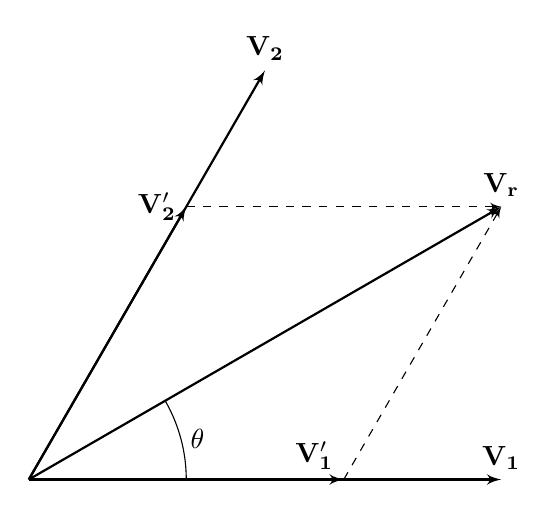
\begin{tikzpicture}[auto, node distance=2cm, >=latex']
            % Define the origin
            \coordinate (O) at (0,0);

            % Define the vectors
            \coordinate (V1) at ({6*cos(0)},{6*sin(0)});
            \coordinate (V2) at ({6*cos(60)},{6*sin(60)});
            \coordinate (V1*) at ({4*cos(0)},{4*sin(0)});
            \coordinate (V2*) at ({4*cos(60)},{4*sin(60)});
            \coordinate (VR) at ({4*cos(0)+4*cos(60)},{4*sin(60)+4*sin(0)});

            % Draw the vectors
            \draw[->, thick] (O) -- (VR) node[midway, above,pos=1] {$\mathbf{V_r}$};
            \draw[->, thick] (O) -- (V1) node[midway, above,pos=1] {$\mathbf{V_1}$};
            \draw[->, thick] (O) -- (V2) node[midway, above,pos=1] {$\mathbf{V_2}$};
            \draw[->, thick] (O) -- (V1*) node[midway, above left,pos=1] {$\mathbf{V_1'}$};
            \draw[->, thick] (O) -- (V2*) node[midway, left,pos=1] {$\mathbf{V_2'}$};

            % Draw Projections
            \draw[->, dashed] (V1*) -- (VR);
            \draw[->, dashed] (V2*) -- (VR);

            % Draw Arc
            \draw (2,0) arc[start angle=0, end angle=30, radius=2] node[midway, right] {$\theta$};

        \end{tikzpicture}
    }
    \caption{Time Interval Calculation}
    \label{fig:til}
\end{figure}

Given the vector \( V_r \), represented by \( V_1 \) and \( V_2 \), the
normalized time durations \( T_A \) and \( T_B \) are calculated as follows:
\[
    V_1' = V_1 \frac{T_A}{T_s}
\]
\[
    V_2' = V_2 \frac{T_B}{T_s}
\]
Using the sine law:
\[
    \frac{V_1'}{\sin \left(\frac{\pi}{3} - \theta\right)} = \frac{V_2'}{\sin \theta} = \frac{V_r}{\sin \frac{2\pi}{3}}
\]
\[
    \frac{V_1 T_A}{\sin \left(\frac{\pi}{3} - \theta\right)} = \frac{V_2 T_B}{\sin \theta} = \frac{V_r T_s}{\sin \frac{2\pi}{3}}
\]
\[
    T_A = \frac{V_r}{V_1} \frac{2}{\sqrt{3}} T_s \sin \left(\frac{\pi}{3} - \theta\right)
\]
\[
    T_B = \frac{V_r}{V_2} \frac{2}{\sqrt{3}} T_s \sin \theta
\]
Magnitude of \( V_1 = V_2 = \frac{2}{3} V_D \)

\noindent
In normalized units, where \( M = \frac{\sqrt{3} V_r T_s}{V_D} \):
\[
    T_A = M \sin \left(\frac{\pi}{3} - \theta\right)
\]
\[
    T_B = M \sin \theta
\]
\( M \) is the modulation index.

\noindent
For the \( N \)-th Sector, \( \theta \rightarrow \theta - (N-1) \frac{\pi}{3}
\):
\[
    T_A = M \sin \left(\frac{N \pi}{3} - \theta\right)
\]
\[
    T_B = M \sin \left(\left(-(N-1) \frac{\pi}{3}\right) + \theta\right)
\]

\subsubsection{Switching Sequence}
Implementing a switching sequence that minimizes switching losses and ensures
smooth transitions between vectors is crucial for the efficiency and
performance of SVPWM. This sequence involves switching between the active and
zero vectors in a manner that reduces the number of switching operations and
distributes the switching events evenly across the phases.\\

The primary goal is to minimize the number of times the switches in the
inverter change states, which helps in reducing switching losses. By doing so,
the overall efficiency of the inverter improves, and the heat generated by
switching operations is minimized. The secondary goal is to ensure that the
transitions between the voltage vectors are smooth, which helps in maintaining
a high-quality output voltage waveform with minimal harmonic distortion.

\begin{table}[ht]
    \centering
    \begin{tabular}{|c|c|c|c|c|c|}
        \hline
        Sector                  & Sequence      & Active Vector 1 & Zero Vector & Active Vector 2 \\ \hline
        $0^\circ - 60^\circ$    & \text{Case 1} & $V1$            & $V0$        & $V2$            \\ \hline
        $60^\circ - 120^\circ$  & \text{Case 2} & $V2$            & $V0$        & $V3$            \\ \hline
        $120^\circ - 180^\circ$ & \text{Case 3} & $V3$            & $V0$        & $V4$            \\ \hline
        $180^\circ - 240^\circ$ & \text{Case 4} & $V4$            & $V0$        & $V5$            \\ \hline
        $240^\circ - 300^\circ$ & \text{Case 5} & $V5$            & $V0$        & $V6$            \\ \hline
        $300^\circ - 360^\circ$ & \text{Case 6} & $V6$            & $V0$        & $V1$            \\ \hline
    \end{tabular}
    \caption{Switching Sequence for Each Sector}
    \label{tab:switching-sequence}
\end{table}

\subsubsection{Gate Pulse Generation}
The gate pulses are generated in a specific manner to achieve these objectives.
When the inverter bridge transitions through different active vectors, the
switching sequence is designed such that only one of the half-bridges changes
its state at any given time. This is achieved by arranging the active and zero
vectors in a specific order, ensuring that the transitions involve only a
single switch change per half-bridge.\\

To determine the optimal switching sequence, the following steps are taken:

\begin{itemize}
    \item \textbf{Sector Division}:The entire space vector plane is divided into six sectors, each spanning 60 degrees. Each sector has a unique combination of active and zero vectors that are used to synthesize the desired output voltage vector.
    \item\textbf{Case Analysis for Each Sector}: For each of the six sectors, a detailed analysis is performed to arrange the active and zero vectors in an optimal sequence. This involves selecting the nearest active vectors to the desired output vector and arranging them along with the zero vectors in a way that minimizes switching operations.
    \item \textbf{Sequence Arrangement}:The active and zero vectors are arranged in a sequence that ensures only one of the half-bridges changes its state at any time. This typically involves transitioning from an active vector to a zero vector, then to the next active vector, and so on. The specific sequence depends on the position of the desired output vector within the sector.
\end{itemize}

\begin{figure}[ht]
    \centering
    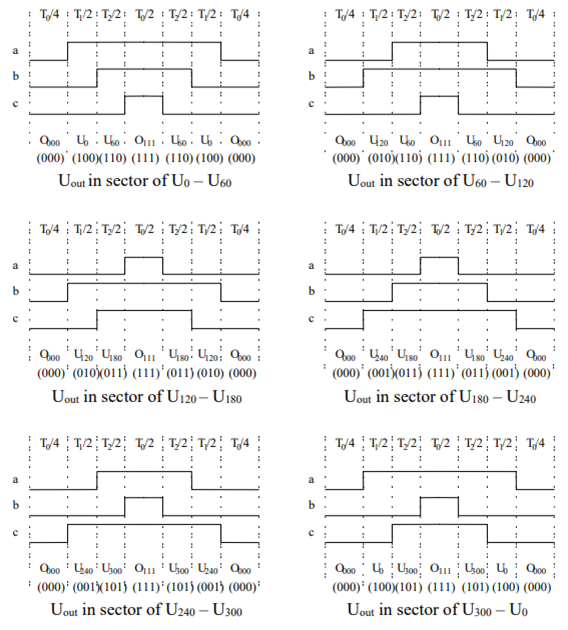
\includegraphics[width=\textwidth]{sequence.png}
    \caption{Gate Pulse Sequence}
    \label{fig:gate_pulse_sequence}
\end{figure}
\section{Matlab/SIMULINK Simulation}
In this section, I will explain the setup-by-steo process I took for building
and Active Front End (AFE) in SIMULINK/MATLAB. This involves creating a
three-phase grid, making a three-phase bridge, implementing a line-tophase
voltage conversion function, and developing a three-phase
Phase-Locked-Loop(PLL) for grid sunchronization. I will also cover the park and
clarke transformations, vector magnitude and angle calculation, current
control, and gate time calculation.

\begin{figure}[ht]
    \centering
    \resizebox{\linewidth}{!}{
        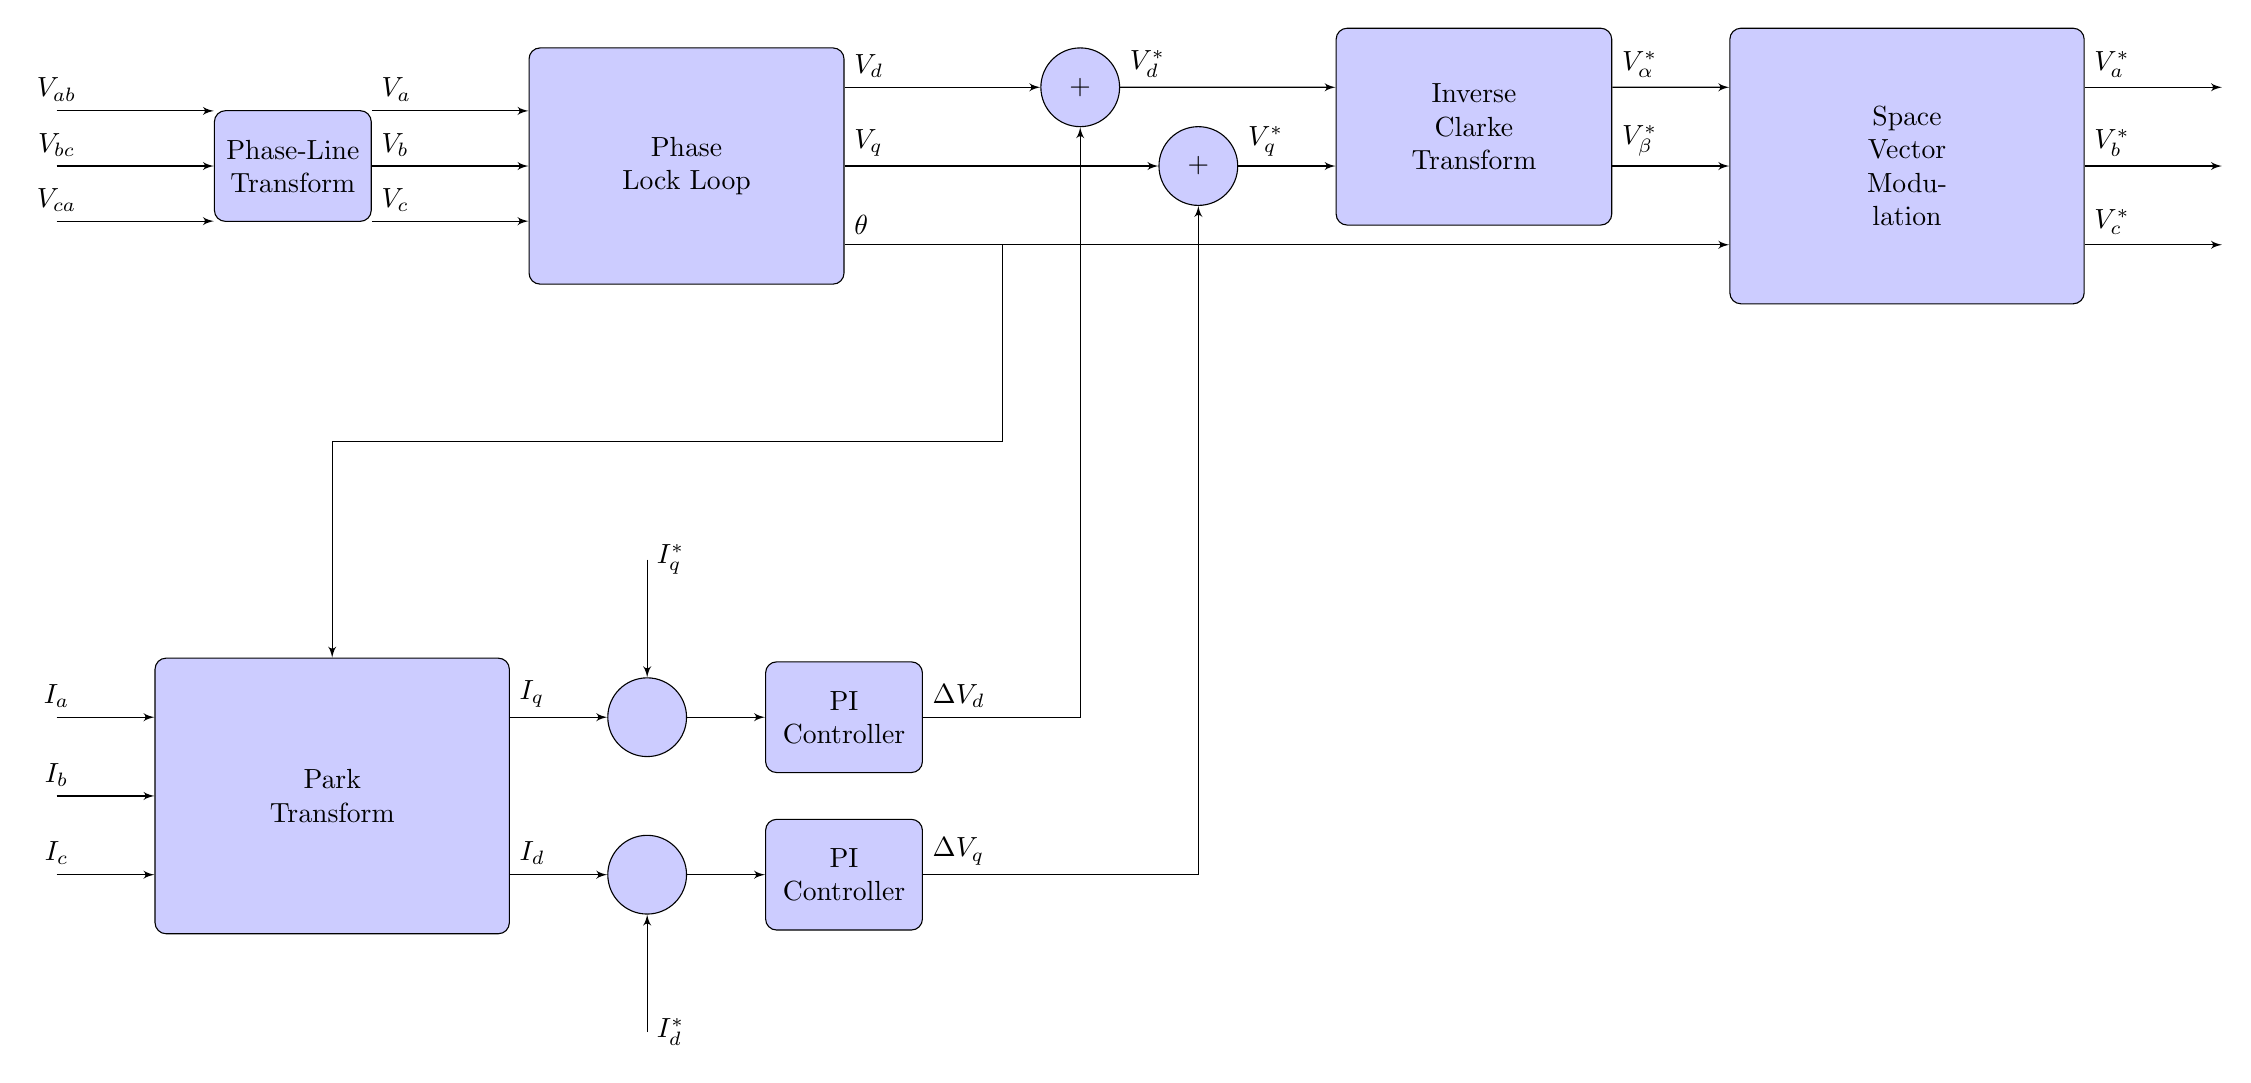
\begin{tikzpicture}[auto, node distance=2cm,>=latex']
            % Nodes
            \node [input, name=Vbc] {};
            \node [input, name=Vab, above of=Vbc,node distance=0.7cm] {};
            \node [input, name=Vca, below of=Vbc, node distance=0.7cm] {};
            \node [block, right of=Vbc,node distance=3cm] (phaseline) {Phase-Line Transform};
            \node [block, right of=phaseline,node distance=5cm, minimum height=3cm, minimum width=4cm] (PLL) {Phase Lock Loop};
            \node [block, right of=PLL,yshift=0.5cm,node distance=10cm, minimum height=2.5cm, minimum width=3.5cm] (iclarke) {Inverse Clarke Transform};

            \node [input, name=Ibc, below of=Vbc, node distance=8cm] {};
            \node [input, name=Iab, above of=Ibc,node distance=1cm] {};
            \node [input, name=Ica, below of=Ibc, node distance=1cm] {};
            \node [block, right of=Ibc, node distance=3.5cm, minimum height=3.5cm, minimum width=4.5cm] (park) {Park Transform};

            \node [sum, name=sumID, right of=PLL, yshift=1cm, node distance =5cm]{$+$};
            \node [sum, name=sumIQ, right of=PLL, node distance=6.5cm]{$+$};

            \node [block, name=svm, right of=PLL, node distance=15.5cm, minimum height=3.5cm, minimum width=4.5cm]{Space Vector Modulation};

            \node [block, name=piID, right of=park, node distance=6.5cm, yshift=1cm]{PI\\Controller};
            \node [block, name=piIQ, right of=park, node distance=6.5cm, yshift=-1cm]{PI\\Controller};

            \node [sum, name=setIQ, left of=piID, node distance=2.5cm]{};
            \node [sum, name=setID, left of=piIQ, node distance=2.5cm]{};

            \node [input, name=Id, below of=setID, node distance=2cm]{};
            \node [input, name=Iq, above of=setIQ, node distance=2cm]{};

            \node [output, name=gb, right of=svm, node distance=4cm]{};
            \node [output, name=ga, above of=gb, node distance=1cm]{};
            \node [output, name=gc, below of=gb, node distance=1cm]{};

            % Connections
            \draw[->] (Vab) node[above]{$V_{ab}$} -- ([yshift=0.7cm]phaseline.west);
            \draw[->] (Vbc) node[above]{$V_{bc}$} -- (phaseline.west);
            \draw[->] (Vca) node[above]{$V_{ca}$} -- ([yshift=-0.7cm]phaseline.west);

            \draw[->] ([yshift=0.7cm]phaseline.east) node[above right]{$V_{a}$} -- ([yshift=0.7cm]PLL.west);
            \draw[->] (phaseline.east) node[above right]{$V_{b}$} -- (PLL.west);
            \draw[->] ([yshift=-0.7cm]phaseline.east) node[above right]{$V_{c}$} -- ([yshift=-0.7cm]PLL.west);

            \draw[->] (Iab) node[above]{$I_{a}$} -- ([yshift=1cm]park.west);
            \draw[->] (Ibc) node[above]{$I_{b}$} -- (park.west);
            \draw[->] (Ica) node[above]{$I_{c}$} -- ([yshift=-1cm]park.west);

            \draw[->] ([yshift=1cm]PLL.east) node[above right]{$V_d$} -- (sumID.west);
            \draw[->] (PLL.east) node[above right]{$V_q$} -- (sumIQ.west);
            \draw[->] (sumID.east) node[above right]{$V_d^*$} -- ([yshift =0.5cm]iclarke.west);
            \draw[->] (sumIQ.east) node[above right]{$V_q^*$} -- ([yshift =-0.5cm]iclarke.west);

            \draw[->] ([yshift=0.5cm]iclarke.east) node[above right]{$V_\alpha^*$} -- ([yshift=1cm]svm.west);
            \draw[->] ([yshift=-0.5cm]iclarke.east) node[above right]{$V_\beta^*$} -- (svm.west);
            \draw[->] ([yshift=-1cm]PLL.east) node[above right]{$\theta$} -- ([yshift=-1cm]svm.west);

            \draw[->] (piID.east) node[above right]{$\Delta V_d$} -|(sumID.south);
            \draw[->] (piIQ.east) node[above right]{$\Delta V_q$} -|(sumIQ.south);

            \draw[->] (setIQ.east) -- (piID.west);
            \draw[->] (setID.east) -- (piIQ.west);

            \draw[->] (Iq) node[right]{$I_q^*$} -- (setIQ.north);
            \draw[->] (Id) node[right]{$I_d^*$} -- (setID.south);

            \draw[->] ([yshift=1cm]park.east) node[above right]{$I_q$} -- (setIQ.west);
            \draw[->] ([yshift=-1cm]park.east) node[above right]{$I_d$} -- (setID.west);

            \draw[->] ([yshift=-1cm,xshift=2cm]PLL.east)--([yshift=-3.5cm,xshift=2cm]PLL.east)-|(park.north);

            \draw[->] ([yshift=1cm]svm.east) node[above right]{$V_a^*$} -- (ga);
            \draw[->] (svm.east) node[above right]{$V_b^*$} -- (gb);
            \draw[->] ([yshift=-1cm]svm.east) node[above right]{$V_c^*$} -- (gc);
        \end{tikzpicture}
    }
    \caption{Active Front End Converter}
    \label{fig:FEC}
\end{figure}

\subsection{Three-phase Grid}
\begin{figure}[h]
    \centering
    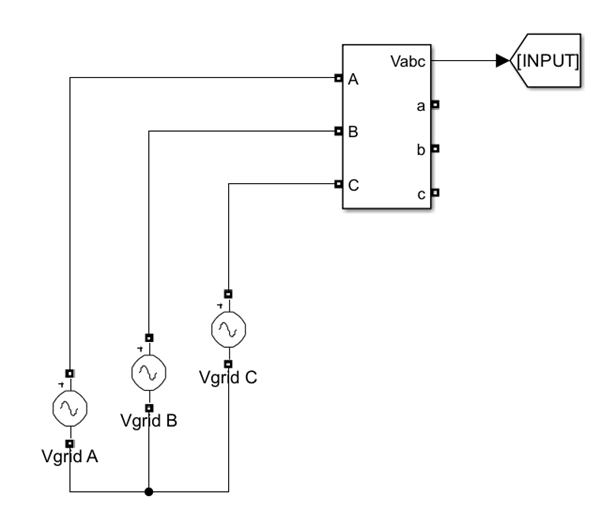
\includegraphics[width=0.5\textwidth]{grid.png}
    \caption{Three Phase Grid in SIMULINK}
    \label{fig:Grid}
\end{figure}
To begin, I created a three-phase grid using SIMULINK's AC source block. This
grid represents the primary input power supply to the system. By connecting
three AC source blocks in a star configuration, I established a three-phase AC
source. Additionally, I added a three-phase VI measurement block to accurately
measure the grid voltage, which I labeled as $INPUT$ to maintain clarity within
the simulation environment.

\subsection{Three-Phase Bridge}
\begin{figure}[h]
    \centering
    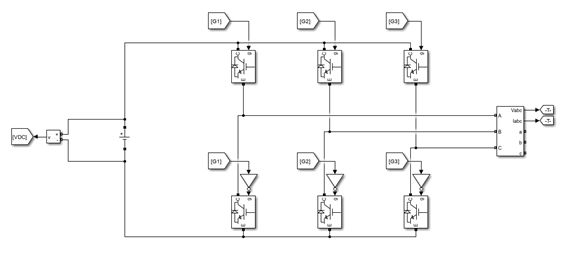
\includegraphics[width=0.8\textwidth]{bridge.png}
    \caption{Front End Conveerter IGBT Bridge}
    \label{fig:Bridge}
\end{figure}
To proceed, I constructed a three-phase bridge using Insulated Gate Bipolar
Transistors (IGBTs) within SIMULINK. Each IGBT gate was labeled as G1, G2, and
G3.\\

To power the bridge, a DC voltage source was added. This source provided the
necessary voltage to drive the IGBTs and maintain stable operation of the
bridge circuit. A voltage measurement block, labeled as VDC, was included to
monitor the DC voltage across the bridge. This measurement block enabled
real-time monitoring and adjustment of the DC voltage level during
simulation.\\

For monitoring the output of the bridge, a three-phase VI measurement block was
connected to the bridge's output terminals. This block facilitated the
measurement and monitoring of both the output voltage (labeled as Vout) and
current (labeled as Iout). These measurements were crucial for the control
system to generate the necessary gate pulses for the IGBTs.

\subsection{Line-To-Phase Voltage conversion}
To apply control algorithms, I needed to convert the measured phase voltages to
line voltages. This involves defining a transformation matrix and implementing
it in a MATLAB function block.

\begin{lstlisting}[style=MATLAB, caption={Phase to Line voltage transformation function}, label={lst:matlab}]
    function [Va, Vb, Vc] = lineToPhase(Vab, Vbc, Vca)
    % Accepts three variables Vab, Vbc, and Vca representing phase voltages
    
    % Combine inputs into a matrix
    V = [Vab, Vbc, Vca];
    
    % Transformation matrix
    T = [2/3, 1/3, 0;
         -1/3, -1/3, 0;
         -1/3, -2/3, 0];
    
    % Calculate phase voltages
    PhaseVoltages = T * V;
    
    % Extract individual phase voltages
    Va = PhaseVoltages(1);
    Vb = PhaseVoltages(2);
    Vc = PhaseVoltages(3);
    end
\end{lstlisting}

\begin{figure}[h]
    \centering
    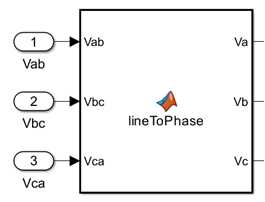
\includegraphics[width=0.5\textwidth]{linefunction.png}
    \caption{Phase-Line Voltage Conversion function}
    \label{fig:phase}
\end{figure}

\subsection{Three-Phase Phase-Locked Loop (PLL)}
The PLL is crucial for accurately measuring the phase and frequency of the grid
voltage, which is essential for generating constant voltages via the Park
transformation. These voltages are subsequently used for current control within
the Active Front End (AFE).\\

I implemented a MATLAB function block in SIMULINK to perform PLL operations.
This function takes line voltages as inputs and outputs park voltages along
with the phase angle ($\theta$).\\

\begin{lstlisting}[style=MATLAB, caption={Three-Phase Phase-Locked Loop}, label={lst:matlab}]
    function [Vd, Vq, theta_o] = PLL(Va, Vb, Vc)
    % Proportional and Integral Controller Parameters
    kp = 28.935; % Proportional gain
    ki = 173610; % Integral gain
    
    % Sampling Time
    dt = 1e-4; % Time step
    
    % Persistent Variables Initialization
    persistent theta; % Phase angle
    if isempty(theta)
        theta = 0;
    end
    
    persistent pid_i; % Integral term of PID controller
    if isempty(pid_i)
        pid_i = 0;
    end
    
    % Park Transformation Matrix
    phi = (2*pi)/3;
    T = [cos(theta), cos(theta - phi), cos(theta + phi);
         sin(theta), sin(theta - phi), sin(theta + phi)] * (2/3);
     
    % Input Vector
    Vabc = [Va; Vb; Vc];
    
    % Park Transformation
    ParkVoltages = T * Vabc;
    Vd = ParkVoltages(1);
    Vq = ParkVoltages(2);
    
    % Error Calculation
    error = Vq;
    
    % PID Controller
    pid_p = kp * error; % Proportional term
    pid_i = pid_i + ki * error * dt; % Integral term
    pid = pid_p + pid_i; % Total PID output
    
    % Frequency Calculation
    omega = 2*pi*50 + pid;
    
    % Phase Angle Integration
    theta = theta + (omega * dt);
    
    % Roll back to zero if theta exceeds 2*pi
    if theta > 2*pi
        theta = 0;
    end
    
    % Output the phase angle
    theta_o = theta;
end
\end{lstlisting}

\subsection{$DQ0-\alpha\beta0$ Transformation}
The newly calculated voltages \( V_d^* \) and \( V_q^* \) are derived from the
output of the current PI loops. These voltages represent the transformed
components in the stationary reference frame after applying the Inverse Clarke
transform, which converts them from the rotating reference frame. This
transformation is crucial for subsequent calculations, such as determining the
timings required for space vector modulation.\\

In the provided MATLAB function block shown in Listing \ref{lst:iclarke}, the
\( DQ \)-\( \alpha\beta \) transformation is implemented using matrix
operations.\\

\begin{lstlisting}[style=MATLAB, caption={Three-Phase Phase-Locked Loop}, label={lst:iclarke}]
    function [alpha, beta] = DQ_AlphaBeta(D, Q, angle)
    % Transformation Matrix
    T = [cos(angle), -sin(angle);
         sin(angle), cos(angle)];
     
    % Input Vector
    DQ = [D; Q];
    
    % AlphaBeta Transformation
    AlphaBeta = T * DQ;
    alpha = AlphaBeta(1);
    beta = AlphaBeta(2);
end
\end{lstlisting}

\subsection{Reference Signal Generator}

\begin{figure}[h]
    \centering
    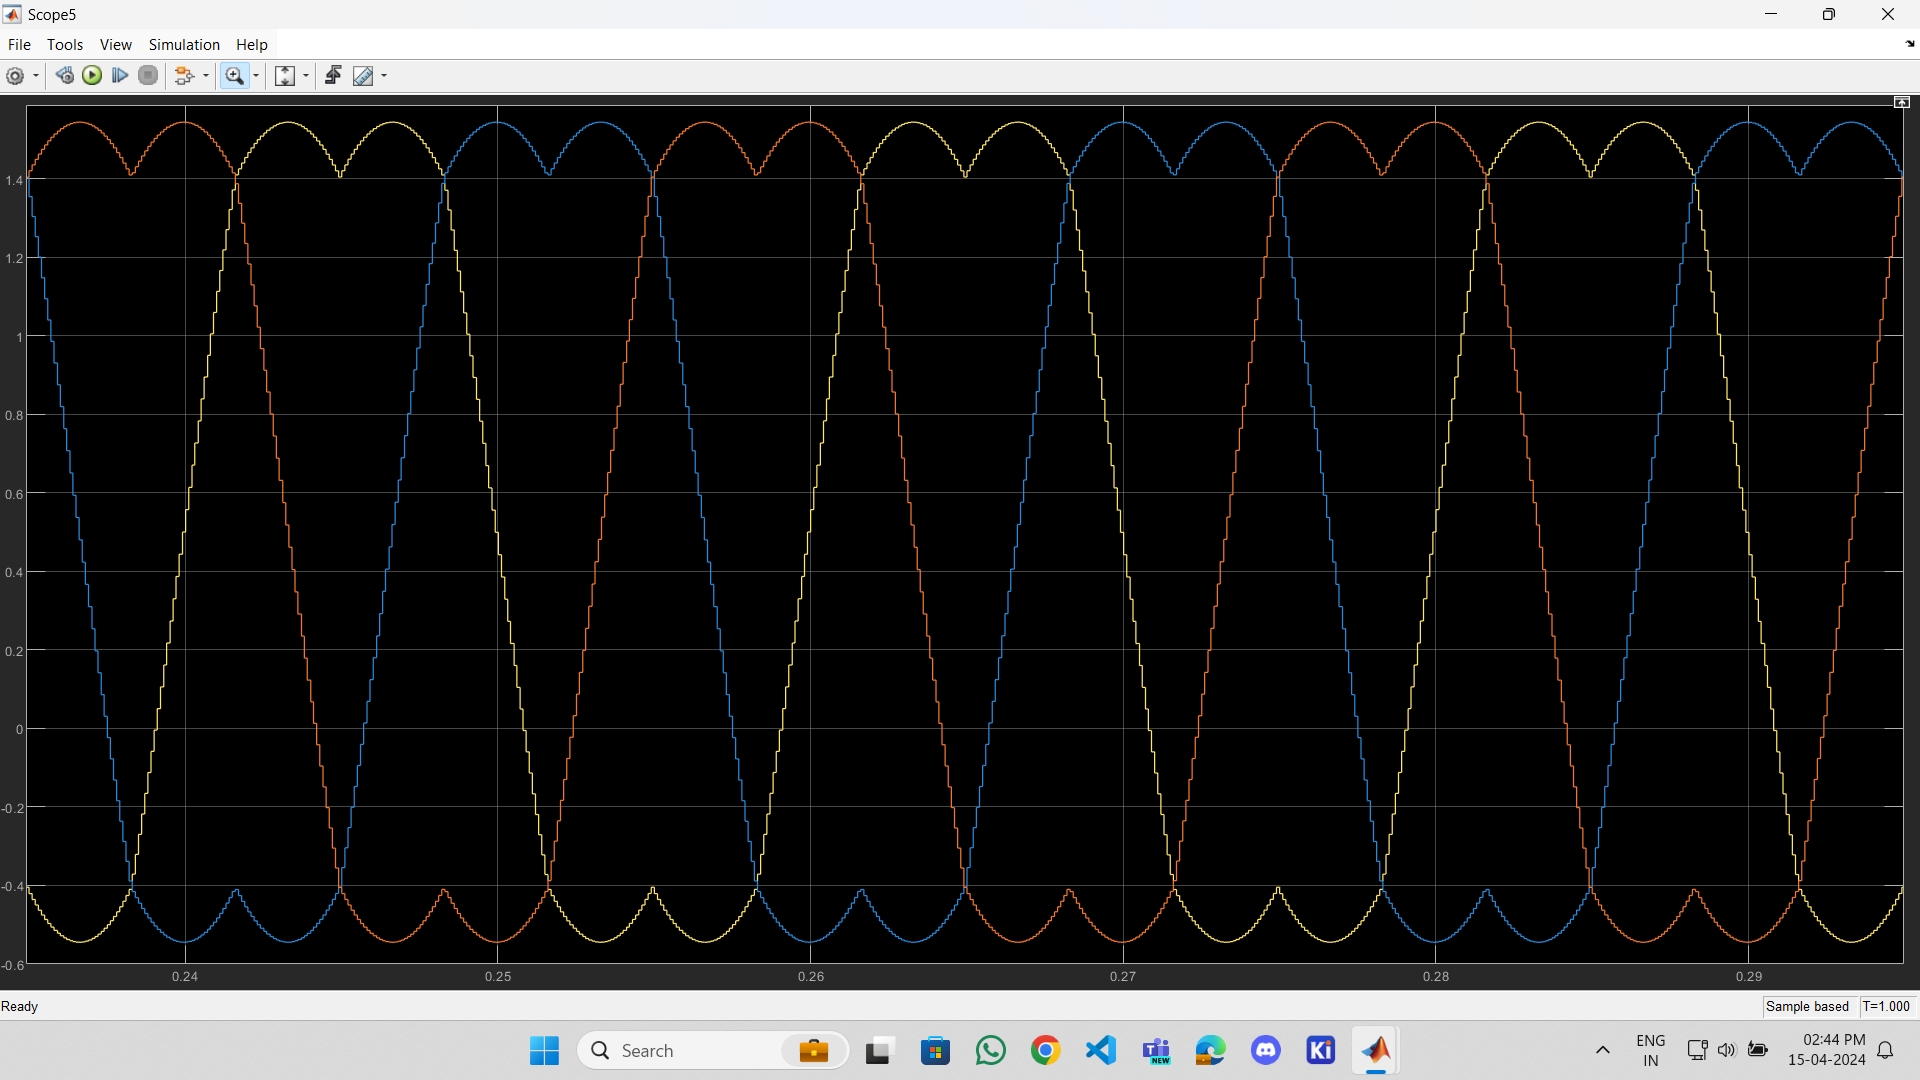
\includegraphics[width=1\textwidth]{matlabsvpwm.png}
    \caption{Space Vector Modulation }
    \label{fig:spaceyfinal}
\end{figure}
The Reference Signal Generator is responsible for generating the reference
signals required for controlling the active front end. These signals,
represented in the \( \alpha\beta0 \) frame, are used to create space vector
modulated signals for the three phases. These modulated signals are compared
with a triangle wave to generate the PWM signal for controlling the IGBT.

\subsubsection{Polar Voltage Conversion}
The new Clarke voltages obtained from the inverse Clarke transform function are
converted to polar voltages. The magnitude of the vector is calculated using
the Pythagorean theorem:
\begin{equation*}
    V = \sqrt{\alpha^2 + \beta^2}
\end{equation*}

To calculate the vector angle, the `atan2` function is used because it provides
angles within the range of \( -2\pi \) to \( 2\pi \):
\begin{equation*}
    \theta = \text{atan2}(\alpha,\beta)
\end{equation*}

\begin{lstlisting}[style=MATLAB, caption={Polar Vector Calculation}, label={lst:polar}]
    V = sqrt(alpha^2 + beta^2);
    
    theta = atan2(alpha,beta);
    if theta < 0 
        theta = theta + 2*pi;
    end
\end{lstlisting}

\subsubsection{Vector Time Calculation}
Using the polar voltages derived from the inverse Clarke transform, the active
vector timings and gate pulse timings are calculated using space vector
modulation. The converter switches through vector states such that only one leg
of the converter changes state at any given time.

\begin{lstlisting}[style=MATLAB, caption={Vector Time Calculation}, label={lst:vector_time}]
    sector = ceil(6 * mod(\theta, 2\pi) / (2\pi));

    TA = V * sin(sector*pi/3 - \theta);
    TB = V * sin(-(sector-1)*pi/3 + \theta);
    T0 = 1 - TA - TB;

    switch sector 
        case 1 
            s1 = TA + TB + T0/2; 
            s2 = TB + T0/2; 
            s3 = T0/2; 
        case 2 
            s1 = TA + T0/2; 
            s2 = TA + TB + T0/2; 
            s3 = T0/2; 
        case 3 
            s1 = T0/2; 
            s2 = TA + TB + T0/2; 
            s3 = TB + T0/2; 
        case 4 
            s1 = T0/2; 
            s2 = TA + T0/2; 
            s3 = TA + TB + T0/2; 
        case 5 
            s1 = TB + T0/2; 
            s2 = T0/2; 
            s3 = TA + TB + T0/2; 
        otherwise 
            s1 = TA + TB + T0/2; 
            s2 = T0/2; 
            s3 = TB + T0/2; 
    end
\end{lstlisting}

In Listing \ref{lst:vector_time}, the MATLAB function calculates the Switch
timings \( s1 \), \( s2 \), and \( s3 \) based on the sector in which the angle
\( \theta \) falls. These timings are crucial for generating the gate pulse
signals that control the IGBTs in the active front end, ensuring proper
modulation of the output voltage.

\subsection{Current Controller}

\begin{figure}[h]
    \centering
    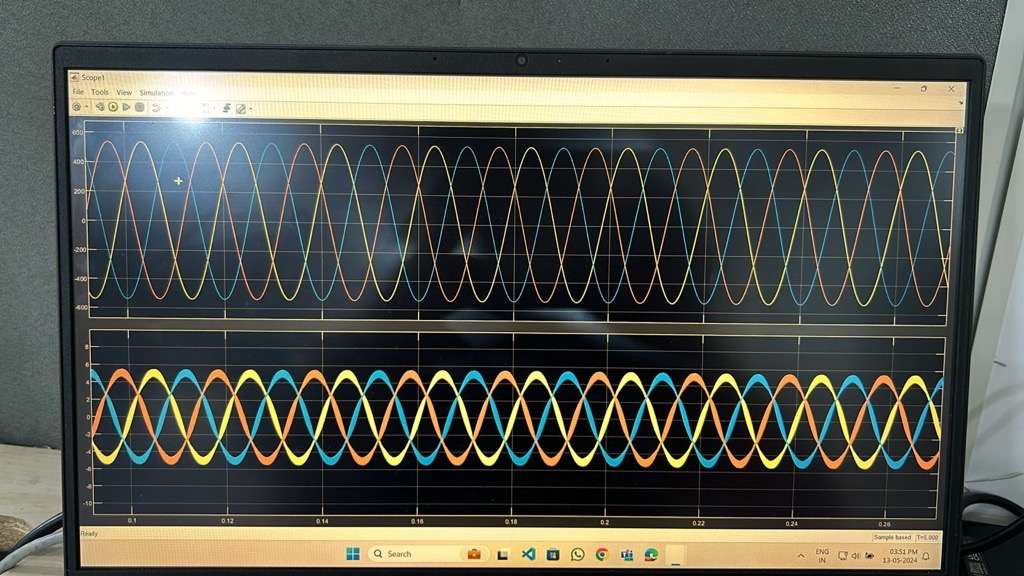
\includegraphics[width=1\textwidth]{Final.jpg}
    \caption{Closed Loop Simulation}
    \label{fig:final}
\end{figure}

The Current Controller plays a crucial role in regulating the output voltage to
achieve precise current control. It operates by converting the line currents
into the DQ-frame of reference and then feeding these components into a PI
controller.

\subsubsection{Park Transformation Function}

The Park transformation function, as shown in Listing \ref{lst:parktransform},
converts the three-phase currents \( I_a, I_b, I_c \) into the DQ-frame of
reference. This transformation aligns the current components \( I_d \) (direct
axis) and \( I_q \) (quadrature axis) with the rotating reference frame, which
is defined by the angle \( \theta \) obtained from the voltage Phase-Locked
Loop (PLL). This alignment ensures that the current remains in phase with the
voltage, thereby achieving a unity power factor.

\begin{lstlisting}[style=MATLAB, caption={Park Transformation}, label={lst:parktransform}]
function [iq, id] = current_transform(ia, ib, ic, theta)
    % Input Vector
    Iabc = [ia; ib; ic];

    % Transformation Matrix
    T = (2/3) * [cos(theta), cos(theta - (2*pi)/3), cos(theta + (2*pi)/3);
                sin(theta), sin(theta - (2*pi)/3), sin(theta + (2*pi)/3)];

    % Park Transformation
    Idq = T * Iabc;
    id = Idq(1);
    iq = Idq(2);
end
\end{lstlisting}

\subsubsection{PI Controller}

The PI Controller, depicted in Listing \ref{lst:picontroller}, operates based
on the \( I_q \) component derived from the Park transformation. It adjusts the
demand \( V_d \) based on the error between the desired \( I_q \) setpoint and
the actual \( I_q \) current. This control loop maintains precise current
levels.\\

\begin{lstlisting}[style=MATLAB, caption={PI Controller}, label={lst:picontroller}]
function Vd_demand = PI_Controller_q(iq, iq_set)
    dt = 1e-4;
    
    persistent pid_i; % Integral term of PID controller
    if isempty(pid_i)
        pid_i = 0;
    end
    
    % Proportional and Integral Controller Parameters
    kp = 47.25; % Proportional gain
    ki = 17010; % Integral gain
    
    % Error Calculation
    error = iq_set - iq;
    
    % PID Controller
    pid_p = kp * error; % Proportional term
    pid_i = pid_i + ki * error * dt; % Integral term
    pid = pid_p + pid_i; % Total PID output
    
    Vd_demand = pid;
end
\end{lstlisting}

These components work in tandem to ensure that the current is precisely
controlled, aligning with the voltage phase to maintain optimal performance and
power efficiency in the active front end.


\chapter{Conclusion and Future scope}
\section{Conclusion}
Throughout my internship at Statcon Electronics India Ltd., I gained extensive
knowledge and practical experience in implementing Space Vector Pulse Width
Modulation (SVPWM). This journey involved understanding and applying various
mathematical transformations, developing control algorithms, and transitioning
from simulation to real hardware implementation.

\noindent
SVPWM offers several advantages over conventional techniques, such as:
\begin{itemize}
    \item \textbf{Higher Efficiency}: SVPWM maximizes the DC bus voltage utilization, leading to improved efficiency in inverter operation. This is crucial for applications where energy efficiency is paramount, such as in renewable energy systems and electric vehicles.
    \item \textbf{Reduced Harmonic Distortion}: By optimizing the switching sequences, SVPWM reduces the harmonic distortion in the output waveforms. This results in cleaner and more stable power delivery, which is essential for sensitive electronic equipment and improving the overall power quality.
    \item \textbf{Improved Power Factor}: SVPWM enables better control over the output voltage and current, contributing to an improved power factor. This is beneficial in reducing energy losses and ensuring that power systems operate closer to their maximum efficiency.
\end{itemize}

\noindent
Moreover, the hands-on experience with simulation tools like MATLAB/Simulink
and practical implementation using STM32F411 microcontrollers has enriched my
understanding of both software and hardware aspects of power electronics. This
dual exposure has equipped me with a holistic view of the challenges and
solutions in modern inverter technology.

\section{Future Scope}
The knowledge and skills developed during this internship have broad
applications in various fields, including:

\begin{itemize}
    \item \textbf{Hybrid Inverters}: Enhancing the efficiency and performance of hybrid inverters. By integrating SVPWM, hybrid inverters can achieve better efficiency and reliability, making them more viable for both residential and commercial energy solutions.
    \item \textbf{Active Front Ends}: Driving DC series motors in trains for power factor correction and voltage regulation. Implementing SVPWM in active front-end converters can lead to significant improvements in power quality and energy savings in traction systems.
    \item \textbf{Battery Charging}: Implementing SVPWM for efficient battery charging systems. With the growing demand for electric vehicles and renewable energy storage, efficient battery charging solutions are critical. SVPWM can contribute to faster and more efficient charging cycles, prolonging battery life and enhancing performance.
    \item \textbf{Electric Vehicle (EV) Drive Systems}: Applying SVPWM in EV drive systems to improve motor efficiency and reduce energy consumption. This can lead to extended range and better performance of electric vehicles, making them more competitive with traditional internal combustion engine vehicles.
\end{itemize}

\noindent
Overall, this internship has been a valuable learning experience, providing me
with the technical expertise and practical skills needed to contribute
effectively to the field of power electronics and embedded systems. The
insights gained have not only broadened my knowledge base but also ignited a
passion for further exploration and innovation in this dynamic and impactful
field.
\begin{thebibliography}{9}
    \bibitem{clarke_transform}
Alpha–beta transformation. (2024, April 19). In Wikipedia. \url{https://en.wikipedia.org/wiki/Alpha%E2%80%93beta_transformation}.

\bibitem{DSP-Based Electromechanical Motion Control}
DSP-Based Electromechanical Motion Control. \url{httpas://kaliasgoldmedal.yolasite.com/resources/MCDSP/UNIT5/Clarke_park.pdf}

\bibitem{R. H. Park}R. H. Park, “Two-reaction theory of synchronous machines – Generalized method of analysis- Part I,” AIEE Trans., Vol. 48, July 1929, pp.716-727

\bibitem{E. Clarke}E. Clarke, Circuit Analysis of AC Power Systems, Vol. I- Symmetrical and Related Components, John Wiley and Sons, New York, 1943.

\bibitem{pid-wikipedia}Proportional–integral–derivative controller. (2024, June 27). In Wikipedia. Retrieved July 6, 2024, from \url{https://en.wikipedia.org/wiki/Proportional%E2%80%93integral%E2%80%93derivative_controller}

\bibitem{feedforward-wikipedia}Feed forward (control). (2024, May 4). In Wikipedia. Retrieved July 6, 2024, from \url{https://en.wikipedia.org/wiki/Feed_forward_(control)}

\bibitem{ziegler-nichols}Ziegler–Nichols method. (2024, March 2). In Wikipedia. Retrieved July 6, 2024, from \url{https://en.wikipedia.org/wiki/Ziegler%E2%80%93Nichols_method}

\end{thebibliography}

\end{document}
